\label{chap:datamodel-dt}


\Cref{chap:dataplat} proposes a generic data architecture of an individual Digital Twin, first through the reference architecture and requirements analysis of \Cref{sec:dataplat-refarch,sec:dataplat-characterization}, and then through the domain-level conceptual schema of \Cref{sec:dataplat-datamodel}, which represents the AGRITECH domain in terms of agents, environments, measurements, and tasks. That architecture, however, focuses mainly on system standardization and the conceptual logical organization of data in it through the proposal of a software infrastructure necessary to sustain the data pipelines collecting and integrating data and the application-level functionality of a hypothetical Digital Twin, but does not address the problem of the conceptual representation of such data in terms of the data model needed to efficiently integrate and query the data flowing through the platform, nor does it address the physical data management systems needed to implement such a model.

A first, natural candidate is to implement the conceptual, object-oriented schema of \Cref{sec:dataplat-datamodel} through a relational model and DBMS, as it is standard practice for structured, schema-first data. However, while a relational DBMS are quite efficient in storing and querying long series of data, such as the ones produced by sensors attached to the physical entity in a Digital Twin, they expose two difficulties that are at the same time characteristic of precision agriculture and , more generally, Digital Twin data. The first concerns the dynamic relationships among entities. Several of the relationships identified in \Cref{sec:dataplat-datamodel}, such as which physical device realizes which logical role, which sector a device is currently assigned to, which thesis is being tested on which sector, do not hold once and for all, but only for a bounded interval of time, and are expected to change repeatedly over a Digital Twin's operational life. Being many-to-many relationships, representing them in a relational model requires dedicated association tables carrying explicit validity intervals, and reconstructing even a moderately complex configuration (i.e. which devices were assigned to which sector, and when) requires joining across several of such tables; as a consequence query performances tend to degrate and maintaining consistence through such table is an extremey time consuming and error-prone task. Furthermore, as these dynamic relationships accumulate, the resulting schema increasingly resembles a network of interconnected entities in which the connections themselves, and their evolution over time, matter as much as the entities they relate: a setting for which the relational model, built around fixed tables and predetermined join paths, is not a natural fit, and towards which graph data models are more directly suited. The second difficulty concerns extensibility: a relational schema fixes, in advance, the set of tables and relationships a schema can represent, so that supporting a new kind of entity, or a new kind of relationship between existing entities, as new functionality is added to the platform, generally requires revising the schema itself -- the same rigidity \Cref{chap:digital_twins,chap:data_oriented_perspective} identified as an obstacle to standardization across evolving, heterogeneous Digital Twin deployments.

These two difficulties motivate considering a graph data model for the entities characterized in \Cref{sec:dataplat-datamodel} and their relationships. Graphs represent entities and relationships uniformly, as nodes and edges, without committing in advance to a fixed schema, so that new entity or relationship types can be introduced without revising an existing structure; and they can represent the temporal evolution of a relationship as a property of the edge realizing it, rather than as an artifact of the physical schema. At the same time, Digital Twin data is not only about the graph of relatively stable entities: it also includes the high-volume, high-frequency time-series data produced by sensors and devices, identified in \Cref{sec:dataplat-characterization} as a defining characteristic of the domain. A graph model well suited to representing entities and their evolving relationships is not, by itself, designed to efficiently store and query such high-frequency time-series; conversely, a data management system optimized for time-series is not designed to represent the rich, evolving topology connecting them to the entities that produce them. This coexistence of graph and time-series data motivates the data model, and the physical system necessary to implement it, presented in this chapter.

The following section presents STGraph, a data model, and its own multistore implementation, that represents slowly evolving entities as a spatio-temporal property graph while managing high-volume, georeferenced time-series through a dedicated time-series store, connecting the two through a shared, efficient representation.
%
Such system has been evaluated in hybrid graph-time-series workloads typical of Digital Twins applications, showing that it can reduce storage footprint and improve ingestion and query performance with respect to temporal graph and multistore baselines.


\section{Introduction}

\label{sec:stgraph_paper}
The unprecedented volume and variety of data generated by the Internet of Things and the rapid adoption of digital twin technologies pose new challenges to data management systems.
On the one hand, modern applications require flexible data models capable of representing evolving spatio-temporal topologies of schemaless entities.
On the other hand, they require optimized mechanisms for ingesting, storing, and querying massive collections of geo-referenced time-series generated by these connected entities.
Relational systems provide mature query capabilities but lack the flexibility required to manage schemaless data.
Graph systems offer expressive representations of complex relationships; however, they are generally not designed to efficiently handle high-volume time-series data.
In this paper, we present \ourapproach, a multistore for spatio-temporal property graphs that combines the expressiveness of spatio-temporal property graph data models with the efficiency required for time-series.
\ourapproach exposes high-volume time-series events as logical graph nodes while persisting and processing them in a dedicated store.
\ourapproach connects graph entities and time-series events through virtual edges, avoids materializing one graph edge per event, and pushes event-local operators to the time-series store.
Our evaluation against temporal graph and multistore baselines shows that this design reduces storage footprint and improves ingestion and query performance on graph-time-series workloads.


The availability of new types of data gives rise to new types of analysis and, consequently, poses new challenges in data management.
The widespread deployment of Internet of Things infrastructures and the rapid adoption of digital twin technologies~\cite{DBLP:journals/cacm/SakrBVIAAAABBDV21} have introduced the need for coupling the analysis of long time-series with semantically rich and complex information.

\begin{example}[Healthcare]
The availability of time-series data on vital signs and physical devices (e.g., pacemakers)~\cite{montagna2020real}, as well as on patients' daily behaviors and medical histories (e.g., treatments, medical conditions), allows physicians to analyze complex cause-and-effect relationships and compare data from multiple patients with similar characteristics.
\end{example}

\begin{example}[Precision agriculture]
Fleets of robots operating in agricultural fields (that belong to a farm, have different crop types, and are managed by different farmers) generate hundreds of georeferenced events per minute~\cite{emmi2023exploiting}.
Integrating these heterogeneous data streams with master data of farms, fields, and crops allow to better understand temporal and spatial activities, transforming precision agriculture systems from mere monitoring tools into proactive, context-aware decision support frameworks.
\end{example}

The examples above pose several data management challenges~\cite{DBLP:journals/sigmod/Tian22}.
The schema-less nature of IoT data requires the adoption of a data model that is both \emph{flexible} and \emph{expressive} to enable the correlation of data that is heterogeneous in nature. 
The ever-changing nature of the data and their spatial characterization require \emph{spatio-temporal query capabilities} and an \emph{efficient versioning} of historical data. 
%(e.g., to know which robots have operated in a field, and when).
The massive volume of long and high-frequency \emph{time-series} requires the ability to \emph{efficiently manage their querying and ingestion}.
The rate at which time-series events are generated can be orders of magnitude greater than that of other types of information, and this crucial factor calls for specialized solutions. 

Relational Database Management Systems (DBMSs) provide a mature and expressive query model supported by decades of optimization research.
However, their schema-first design is less suitable for applications with rapidly evolving, heterogeneous, or semi-structured data, as in IoT and digital twin scenarios.
Moreover, although relational systems can store temporal data, they are not designed for high-rate ingestion or analytical processing of massive time-series measurements.
Graph data models offer an attractive alternative, combining expressive traversals with schema-optional flexibility.
They naturally capture complex relationships among entities and support evolving schemas, making them well suited for semantically rich, interconnected, temporal, and spatial data.
Nevertheless, graph DBMSs are not optimized for dense event streams, where workloads are dominated by sequential writes, time-based filtering, and aggregation.
Conversely, time-series DBMSs support high-throughput ingestion and efficient time-oriented queries over large event collections.
Their data model and query capabilities, however, remain specialized for time-series workloads and lack the expressive power needed to model complex semantic relationships among heterogeneous entities.

These complementary strengths and limitations motivate a multistore architecture~\cite{DBLP:journals/csur/BestaGPFPBAH24,DBLP:journals/sigmod/BonifatiOTVYZ24}, where each database system is responsible for the workload it is designed to support.
However, simply placing a graph DBMS next to a time-series DBMS is not sufficient: applications still need a single graph abstraction, graph traversals must cross the store boundary without materializing one edge per event, and selections, projections, and aggregations over events must be pushed to the time-series store without changing query semantics.
The novelty of \ourapproach lies in this cross-store graph/time-series boundary: time-series events remain logical graph nodes and are reached through virtual graph edges, while their physical storage, ingestion, and event-local computation are delegated to TS.

\begin{figure}[t]
\centering
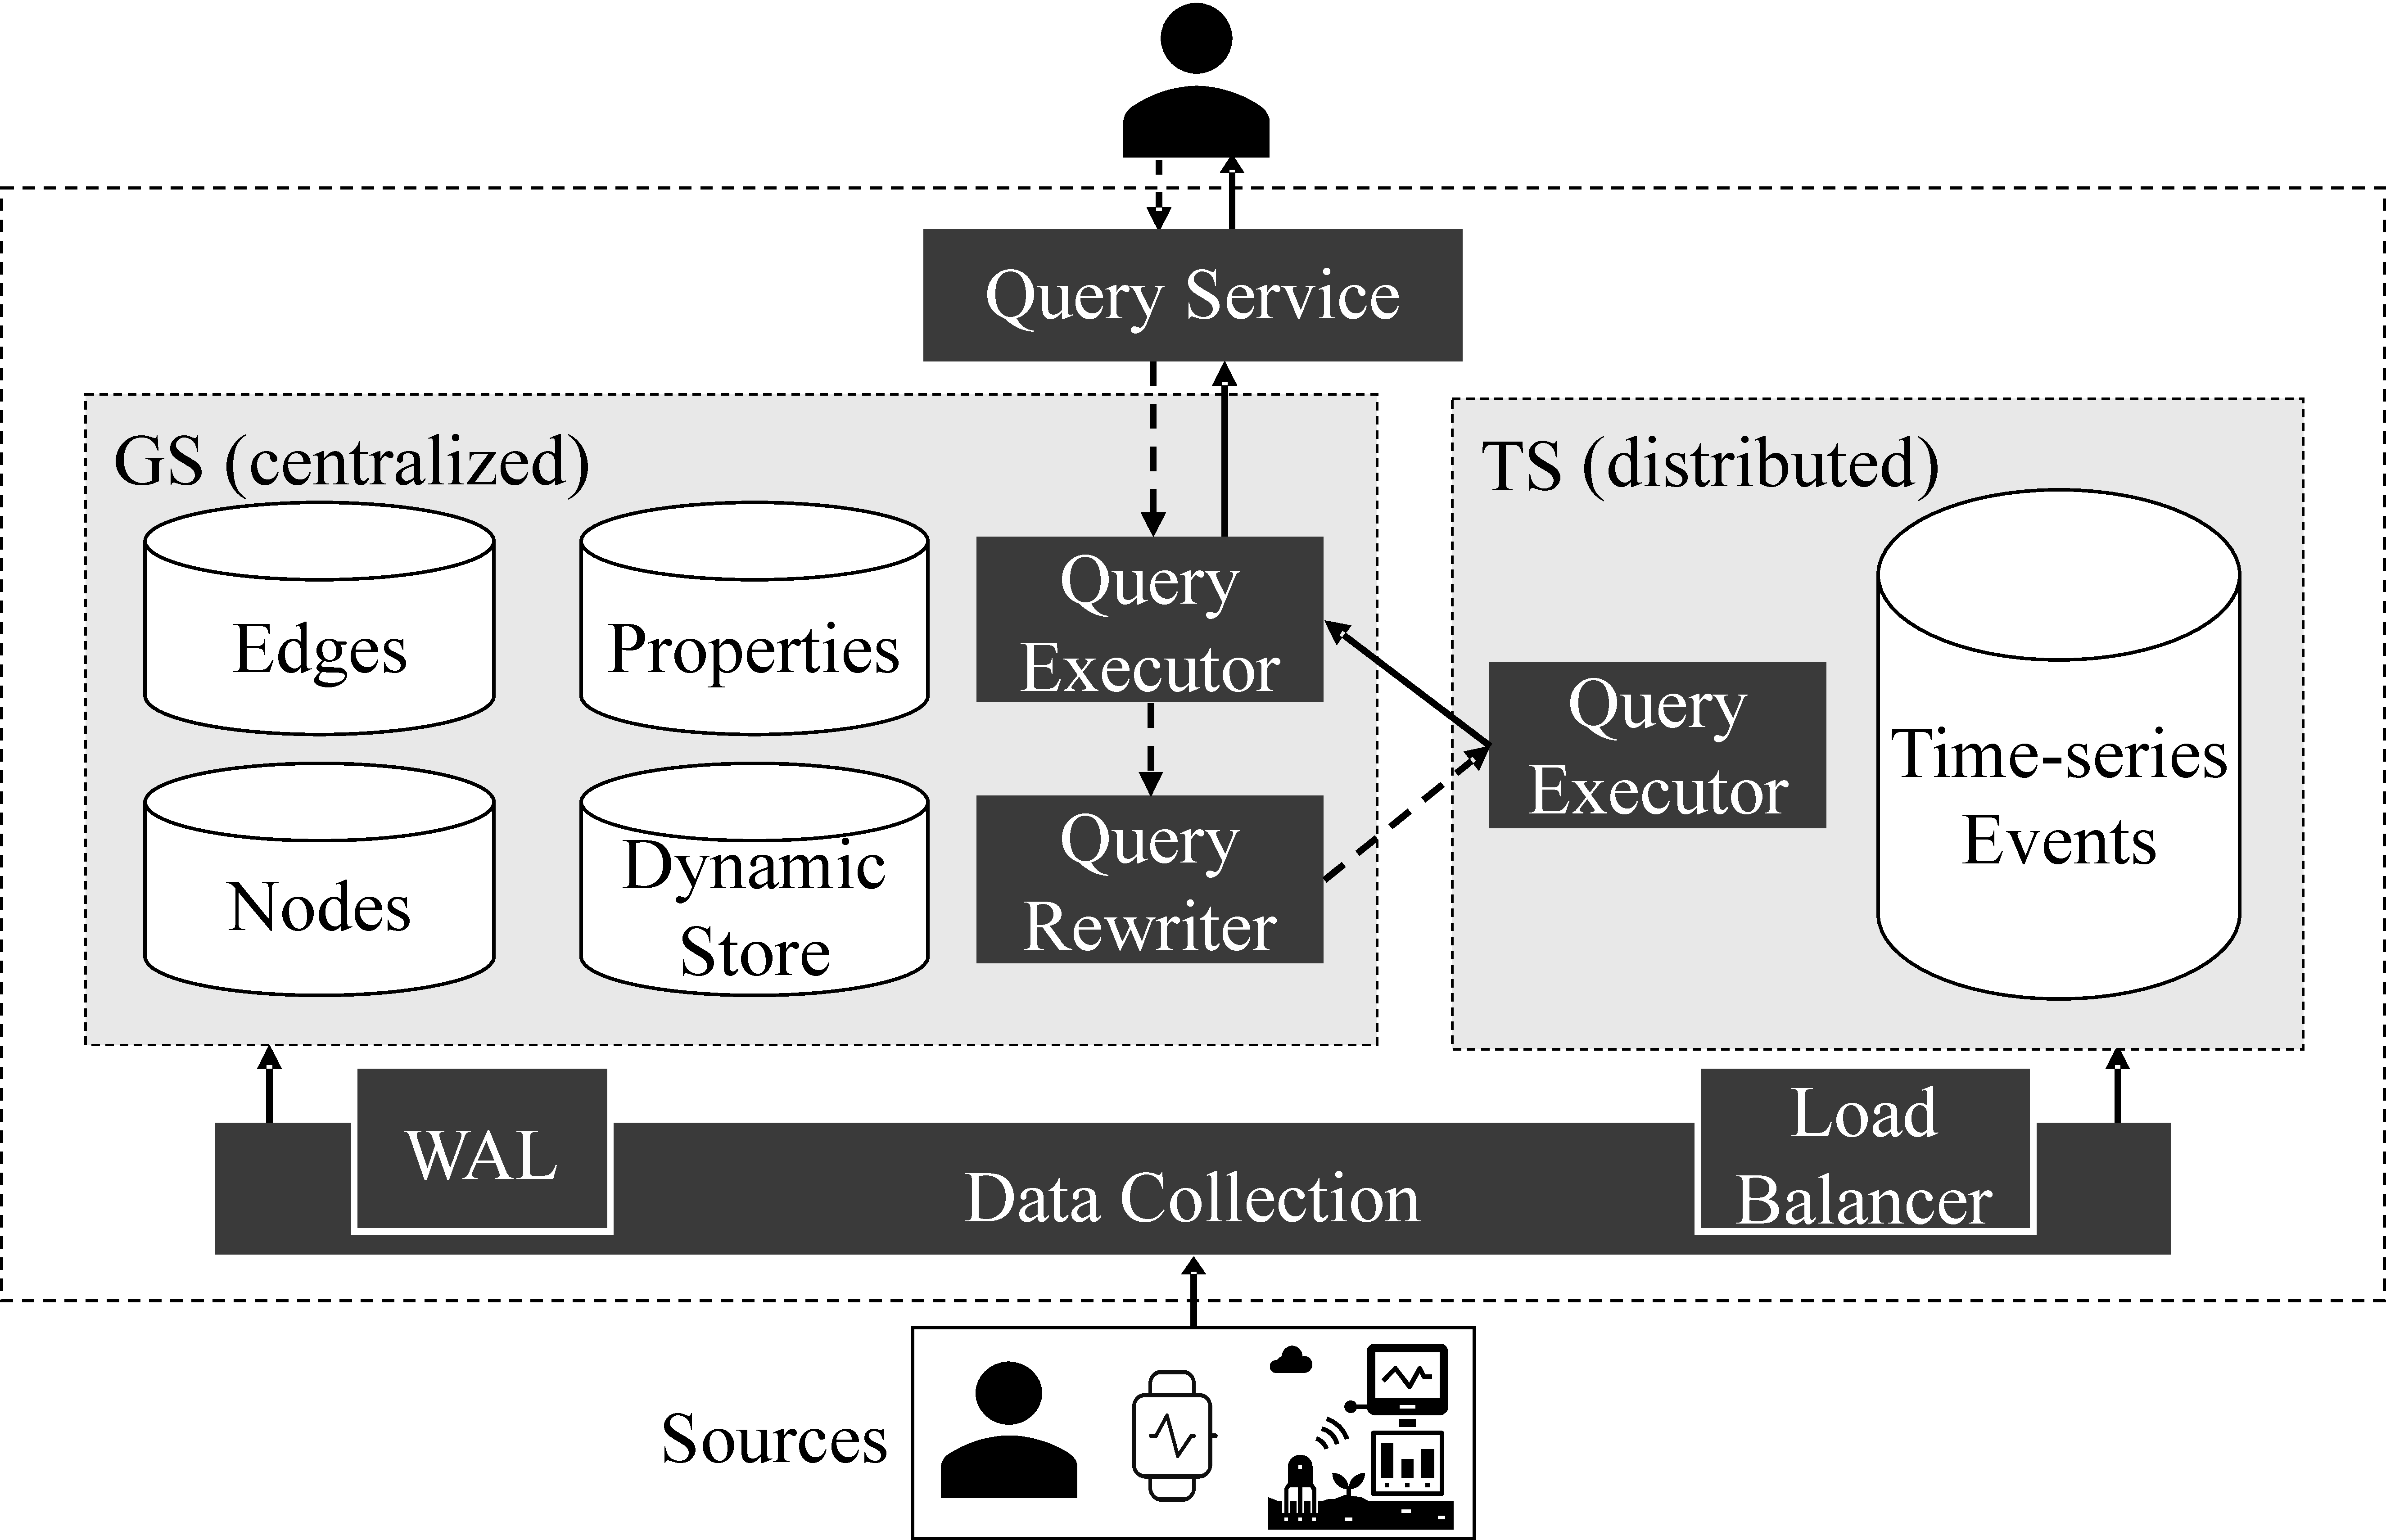
\includegraphics[scale=0.10]{parts/architectures/images/architecture.pdf}
\caption{\ourapproach: straight arrows represent data flows, while dashed arrows represent query-rewriting flows.}
\label{fig:overview}
\end{figure}

\paragraph{Overview and contributions}
We introduce \ourapproach (\Cref{fig:overview}), a multistore for managing spatio-temporal property graphs containing both slowly evolving entities and high-volume geo-referenced time-series events.
From the logical perspective, all data are queried as nodes, edges, and properties.
This choice is taken since graphs natively support interconnected, schemaless and evolving data; evolution is modeled by versioning graph entities with temporal validity and by supporting temporal traversal.
Physically, \ourapproach separates the workload between a Graph Store (GS), which stores materialized graph entities and relationships, and a Time-series Store (TS), which stores events.
The key design point is that events are exposed as graph nodes but are not materialized in GS: they are reached through virtual edges generated during traversal, and event-local predicates, projections, and aggregations are compiled into TS requests.
%, providing a unified abstraction that combines expressive graph querying with scalable time-series management.
At the bottom of \Cref{fig:overview}, data sources upsert data through the ``Data Collection'' service, which is responsible for dispatching the data to either GS or TS.
Uploading data to TS does not require interaction with GS (and vice versa), enabling fully independent management of static/dynamic data.
At the top of \Cref{fig:overview}, users query the spatio-temporal property graph through the ``Query Service'', which interprets the incoming query and transforms it into a query plan that is forwarded to the ``(GS)  Query Executor.''
During graph traversal, if the query requires data from TS, the ``(GS)  Query Executor'' invokes the ``Query Rewriter,'' which translates and pushes the query down to the ``(TS) Query Executor.''
Finally, results are shuffled and aggregated by the ``(GS)  Query Executor.''
%,'' which returns them to the ``Query Service.''

The contributions of \ourapproach are the following.
\begin{enumerate}[label=(\roman*)]
    \item A spatio-temporal property graph abstraction in which time-series events are treated as logical graph nodes, while their physical representation remains in a time-series store.
    \item A multistore storage layout that connects GS and TS through shared identifiers and virtual edges, avoiding the materialization of one graph edge per event while preserving graph traversal semantics.
    \item Cross-store query optimization that pushes event-local selections, projections, and decomposable aggregations to TS and combines their results in GS.
    \item An experimental evaluation against (temporal) graph and multimodel baselines, showing lower storage footprint and faster ingestion/query execution on graph-time-series workloads.
\end{enumerate}

The paper is organized as follows.
\Cref{sec:related} compares \ourapproach with the state-of-the-art contributions.
\Cref{sec:formal} defines the spatio-temporal property graph.
\Cref{sec:stgraph} introduces the multistore storage layout while
\Cref{sec:query} describes the query execution and optimization.
\Cref{sec:exp} extensively tests \ourapproach.
\Cref{sec:conclusion} draws the conclusion and future research directions.

\section{Related Work}\label{sec:related}
The management of schemaless, evolving, and time-series data has received significant attention.
Existing systems can be grouped into single-model, which optimize either time-series or graph workloads, and multimodel/multistore, which combine multiple models but do not provide native cross-store graph traversal over time-series.

In summary, prior systems provide either efficient time-series storage without graph-native traversal, temporal graph management without scalable event ingestion, or multimodel integration through middleware.
\ourapproach does not expose time-series data merely as external attributes, views, or relational extensions, but it makes time-series events logical graph nodes, linking them to GS nodes through virtual edges, and pushes event-local operators down to TS during traversal between GS and TS.
\subsection{Single model solutions}

\subsubsection{Time-series}
Time-series DBMSs have gained popularity with the rise of IoT and digital twins applications in recent years~\cite{DBLP:journals/tkde/JensenPT17}.
Time-series DBMSs usually rely on indexes, such as Log-Structured Merge Trees (LSM-Trees)~\cite{DBLP:journals/acta/ONeilCGO96}, which buffer write operations in memory and flush them to disk in batches, drastically reducing the number of disk accesses and thus achieving exceptional ingestion performance.
%Compaction policies are then progressively performed to organize data as it is flushed to disk.
InfluxDB\footnote{https://www.influxdata.com/} is among the most widely adopted time-series DBMSs.
InfluxDB's primary focus lies in the efficient storage and retrieval of high-volume time-series, rather than in modeling the underlying entities.
Several solutions have been proposed in the literature to address time-series data, such as Apache IoTDB~\cite{DBLP:journals/pvldb/0018HQ00MFZ0ZKJ20}, AsterixDB~\cite{DBLP:journals/pvldb/AlsubaieeAABBBCCCFGGHKLLOOPTVWW14}, and Gorilla~\cite{DBLP:journals/pvldb/PelkonenFCHMTV15}.
Within these, AsterixDB is a shared-nothing distributed big data management system designed to efficiently manage large volumes of semi-structured data.
It adopts a flexible data model based on nested, schema-less records and organizes information into datasets stored on LSM-tree-based storage structures.
%Each dataset is indexed and hash-partitioned across the nodes of the cluster. % using a primary key.

Overall, time-series DBMSs provide the physical properties required by high-rate event workloads, but they do not expose events as part of a rich graph topology and therefore cannot directly express graph traversals over the entities that produce those events.

\subsubsection{(Temporal) Graph}
Graph DBMSs are well-suited for managing highly interconnected environments.
%Their data layout often relies on an index-free adjacency principle that enables efficient relationship navigation via direct neighbor access, making path traversal operations highly efficient.
Neo4J~\cite{Neo4J2025} employs a storage layout built on an index-free adjacency data structure.
However, it does not offer native support for temporal data and its performance tends to degrade when time-series events are represented as ordinary graph nodes and edges.
Recent works have exploited LSM-trees for scalable management~\cite{DBLP:journals/pacmmod/MoLWL25,DBLP:journals/corr/abs-2411-06392}.
However, they are not temporal graphs since they lack versioning.

Debrouvier et al.~\cite{DBLP:journals/vldb/DebrouvierPPSV21} provide a classification of temporal graphs with respect to how temporal information is managed and queried.
%and temporal query semantics:
\textit{Duration-labeled}~\cite{DBLP:journals/tkde/WuCKHHW16}: each edge is annotated with a duration of the relationship.
% between two nodes. 
%At a certain time, a node is considered valid if it participates in at least one edge that is valid at that time.
%This approach is mainly used for scheduling problems, where some shortest path has to be computed and they entail a fixed time granularity.
\textit{Interval-labeled}~\cite{DBLP:journals/vldb/DebrouvierPPSV21}: each node/edge is annotated with a validity interval.
%these temporal graphs could be seen as a generalization of duration-labeled graphs, in which each node/edge is annotated with a validity interval.
This solution allows for a non-fixed time granularity and additional temporal query semantics at the cost of a storage overhead.
\textit{Snapshot-based}~\cite{DBLP:journals/tkde/SemertzidisP19,DBLP:journals/tos/MiaoHLWYZPCC15,DBLP:journals/tlsdkcs/Massri0PM23,DBLP:journals/pvldb/HouZWLJWD24}: represent the graph as a sequence of discrete snapshots at different interval times.
%
Hybrid solutions, such as Copy+Log~\cite{DBLP:journals/tos/MiaoHLWYZPCC15}, $\delta$-Copy+Log~\cite{DBLP:journals/tlsdkcs/Massri0PM23}, and Anchor+Delta~\cite{DBLP:journals/pvldb/HouZWLJWD24}, have been introduced to optimize delta updates of snapshots.
%
Despite each approach optimizes its predecessor through redundancy reduction, snapshot-based representations entail significant storage overhead, which limits their scalability when managing highly dynamic data and large-scale graphs. 

To the best of our knowledge, AeonG~\cite{DBLP:journals/pvldb/HouZWLJWD24} is the state of the art for temporal graphs.
Its Anchor+Delta design balances storage efficiency and query performance by reducing redundant data and limiting read amplification during temporal queries.
% Additionally, the evaluation of AeonG is restricted to relatively small datasets, focusing primarily on small-range and point temporal queries.
With respect to T-GQL~\cite{DBLP:journals/vldb/DebrouvierPPSV21}, Clock-G~\cite{DBLP:journals/tlsdkcs/Massri0PM23}, and AeonG~\cite{DBLP:journals/pvldb/HouZWLJWD24}, \ourapproach follows interval-labeled temporal semantics but targets a different systems problem: time-series events remain queryable as graph nodes while being stored and processed in a dedicated TS backend.

\subsection{Multimodel and multistore solutions}
\subsubsection{Multimodel}
Graphix~\cite{DBLP:conf/icde/Galvizo024} extends AsterixDB with interconnected views over time-series data.
Nonetheless, Graphix does not natively support temporal graphs and relies on logical views over AsterixDB records rather than on a graph/time-series storage split with virtual traversal edges.
Hygraph~\cite{DBLP:conf/edbt/Ammar0BR25} integrates graphs and time-series in a hybrid in-memory data structure.
Time-series are represented as node properties; however, this prevents the possibility to link and assign properties to single events.% and introduces operators to create graph overlays from time-series data.
Being in-memory, Hygraph provides fast graph ingestion but is limited by main-memory capacity and not persistent.% multistore execution.


\subsubsection{Multistore}
AGTS is a multistore solution based on PostgreSQL~\cite{DBLP:conf/sigmod/StonebrakerR86} extended with Apache AGE\footnote{https://age.apache.org/}, TimescaleDB\footnote{https://www.tigerdata.com/}, and PostGIS\footnote{https://postgis.net/}.
PostGIS enhances PostgreSQL with spatial capabilities, TimescaleDB introduces efficient time-series data management via hypertables, and Apache AGE introduces graph capabilities through a hybrid query language (SQL functions that parse Cypher syntax).
Graph data is implemented as logical abstractions on top of PostgreSQL's relational storage model, where each node and edge label is mapped to a corresponding relational table (graph traversals are executed through relational operators rather than native graph-processing mechanisms).

\section{Spatio-temporal property graph}\label{sec:formal}

A spatio-temporal property graph extends the traditional property graph, incorporating both temporal and spatial dimensions.

\begin{definition}[Property graph]\label{def:pg}
A property graph is a tuple:
$G = (N, E, L, P, \ell, \rho)$
where: $N$ is the set of nodes, $E \subseteq N \times N$ is the set of directed edges, $L$ is the set of labels, $P$ is the set of key-value properties, $\ell: N \cup E \to L$ maps each node/edge to a label, $\rho: N \cup E \to 2^P$ maps each node/edge to a set of key-value properties.
\end{definition}
For the sake of brevity, in the remainder of the paper we will refer to node/edge labels and properties using the dot notation (e.g., $n.name$ for the name property of node $n$ and $n.label$ for the $\ell(n)$).

Given the temporal domain $\mathbb{T}$ and the set of spatial objects $\mathbb{S}$, we extend \Cref{def:pg} to a spatio-temporal property graph.

\begin{definition}[Spatio-temporal property graph]\label{def:stg}
A spatio-temporal property graph $G^{st} = (N, E, L, P, \ell, \rho, \ftemporal)$ extends a property graph $G$, where:
$\ftemporal: N \cup E \cup P \to \mathbb{T}^2$ assigns temporal interval validity $[from, to)$ (with $from < to$) to nodes, edges, and properties, enabling an interval-labeled temporal graph; and
$\prop{location}{x} \in P$ is a property that assigns a spatial object $x \in \mathbb{S}$ to nodes and edges.
\end{definition}

Note that (i) node/edge validity must include the validity of its properties, and properties with the same key belonging to same entity cannot have overlapping validity; and (ii) $\texttt{location}$ is a property and not a first-class citizen since nodes/edges can change locations over time (e.g., a person changing the home address).

\begin{figure}[t]
    \centering
    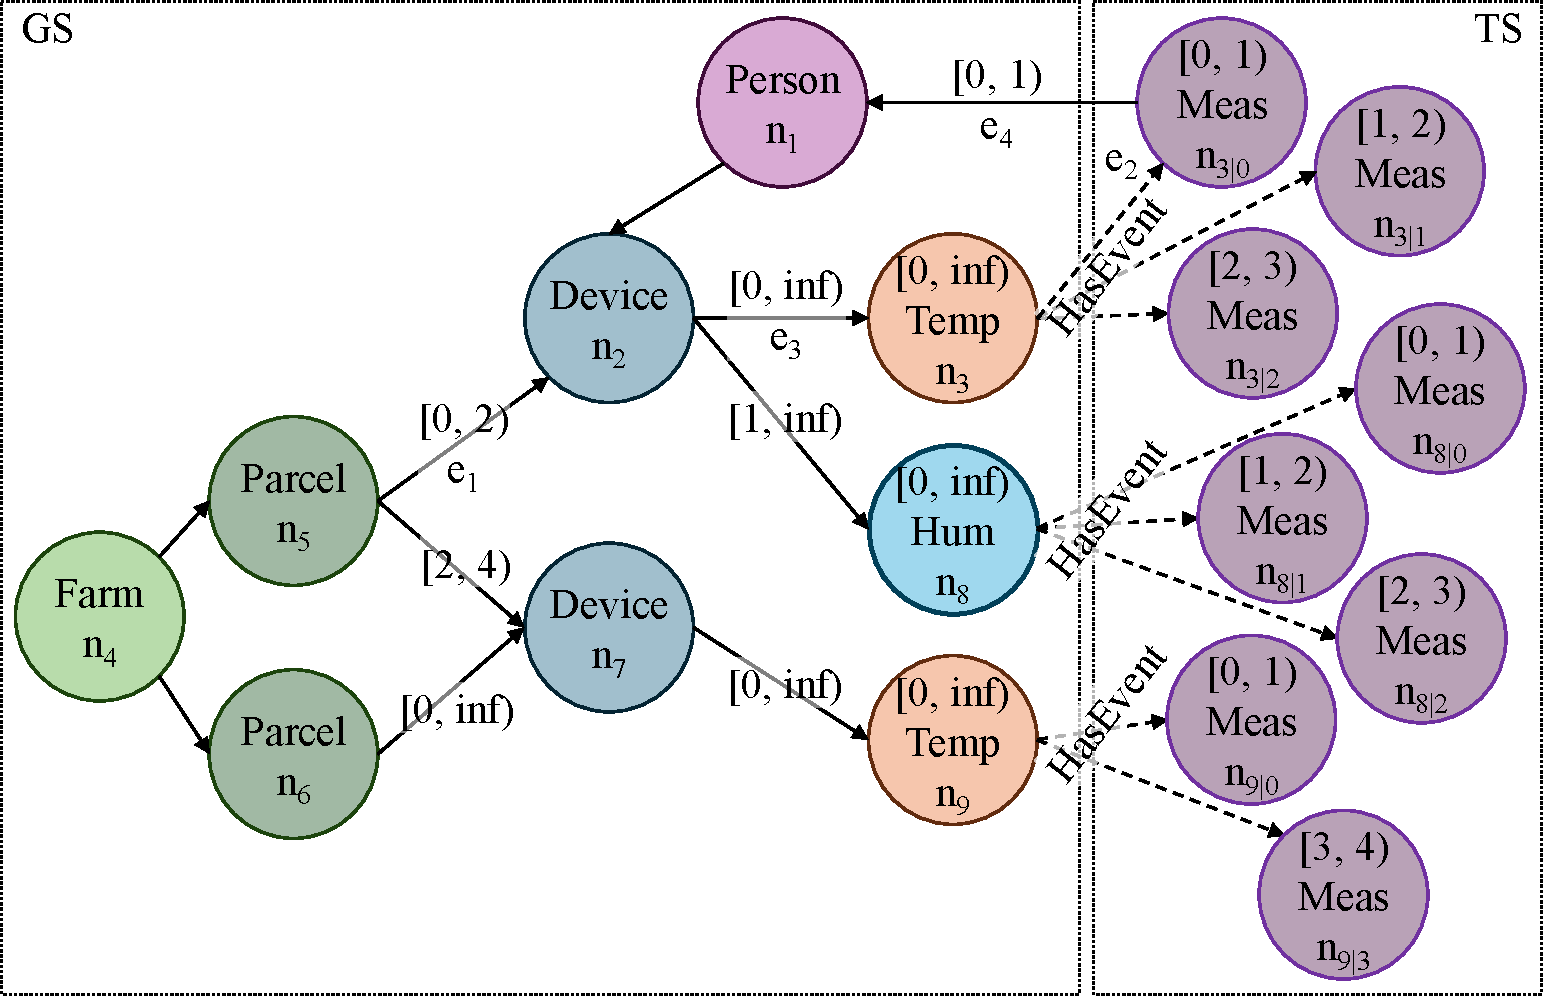
\includegraphics[scale=.32]{parts/architectures/images/example.pdf}
    \caption{Example of a spatio-temporal property graph.
    Different colors represent different node labels. 
    Temporal validity is reported; if omitted, the validity is $(-\inf, \inf)$.
    Node $n_1$ ($``Alice"$, with label \lbl{Person}) is the owner of $n_2$ ($``Device~1"$, \lbl{Device}) (e.g., a weather station) producing two time-series $n_3$ ($``Temp~1"$, \lbl{Temperature}) and $n_8$ ($``Hum~1"$, \lbl{Humidity}).
    $n_4$ ($``Farm~1"$, \lbl{Farm}) is composed of $n_5$ ($``Parcel~1"$, \lbl{Parcel}) and $n_6$ ($``Parcel~2"$, \lbl{Parcel}) that share $n_7$ ($``Device~2"$, \lbl{Device}) producing a time-series $n_9$ ($``Temp~2"$, \lbl{Temperature}).
    $n_5$ also contains $n_2$.
    Edges with label \lbl{HasEvent} are dynamically generated at query time.}
    \label{fig:example}
\end{figure}

\begin{example}
Let $G^{st}$ represent a spatio-temporal property graph modeling \Cref{fig:example}.
The set of nodes $N$ contains $n_2$ (a weather station), $n_5$ (a parcel), and $n_{3|0}$ (a measurement).
The set of edges $E$ contains $e_1 = (n_5, n_2)$ and $e_2 = (n_3, n_{3|0})$.
Examples of labels, properties, and temporal validity are:
\[
\begin{aligned}
n_5.label = \lbl{Parcel}&,\quad e_2.label = \lbl{HasEvent}\\
\rho(n_5) = \{\prop{name}{``Parcel~1"}&,\prop{location}{Polygon(\ldots)}\}\\
\rho(n_{3|0}) = \{\prop{value}{16}&,\prop{unit}{``C"},\prop{location}{Point(\ldots)}\}\\
\ftemporal(n_{3|0}) = [0,1)&,\quad \ftemporal(e_1)= [0,2)
\end{aligned}\]
%\rho(n_2) = \{\prop{name}{``Device~1"}&,\prop{type}{``Weather~Station"}\}\\
\end{example}

\subsection{Operators and query plan}

% We distinguish between the operators necessary to build the spatio-temporal property graph and those used to query it.

% \subsubsection{Versioning the graph}

% Building and versioning the spatio-temporal property graph is based on the following operators.
% \begin{enumerate}
%     \item $\textsf{create}(n)$ (creating a node) adds $n$ to the graph (i.e., $G^{st}.N = G^{st}.N \cup \{n\}$) with a time period $\ftemporal(n)=[from, to)$.
%     Unless otherwise specified, $to = \inf$.
%     \item $\textsf{create}(e)$ (creating an edge) adds $e = (v_1, v_2)$ to the graph (i.e., $G^{st}.E = G^{st}.E \cup \{e\}$) with a time period $\ftemporal(e)=[from_e, to_e)$, where $\ftemporal(e)$ is bounded by the time spans $\ftemporal(v_1)=[from_{v_1}, to_{v_1})$ and $\ftemporal(v_2)=[from_{v_2}, to_{v_2})$.
%     Formally, $from_e \ge max(from_{v_1}, from_{v_2})$ and $to_e \le min(to_{v_1}, to_{v_2})$.
%     Unless otherwise specified, $to_e = \inf$ (i.e., it has no end validity).
%     \item $\textsf{upsert}(x, p)$ (update/add a/to node/edge $x$ with a property $p$) adds $p$ to the graph (i.e., $G^{st}.P = G^{st}.P \cup \{p\}$) with a time period $\ftemporal(p)=[from_p, to_p)$, where $\ftemporal(p)$ is bounded by $\ftemporal(x)=[from_x, to_x)$.
%     Formally, $from_p \ge from_x$ and $to_p \le to_x$.
%     Note that (i) if $x$ already contains a property $p'$ with the same key, $p'.to$ is set to $p.from$; and (ii) adding a property does not update the validity of the node/edge (since its validity could be longer than that of the single property (but the property cannot exceed the validity of the node/edge to which it belongs).
%     \item $\textsf{delete}(x)$ (deleting a node/edge/property) changes its temporal validity from $\ftemporal(x) = [from, to)$ to $\ftemporal(x) = [from, to')$, where $to' < to$.
%     When a node is deleted, all its edges and properties are deleted as well.
%     When an edge is deleted, all its properties are deleted as well.
% \end{enumerate}
% To be valid, a spatio-temporal property graph requires the above temporal constraints to be satisfied, but it does not require any spatial constraint (e.g., a weather station installed in a farm can ``cover'' a surface larger than the farm).

%Creating an element inserts a record with validity $[from,\inf)$ unless a \textit{to} timestamp is provided.
%Deleting an element closes its validity interval by setting its $to$ timestamp.
%Updating a property closes the validity of the previous property record and creates a new property record with the new value and validity.
%Note that these operators do not require materializing full graph snapshots or maintaining separate delta structures.
%For instance, in \Cref{fig:example}, $n_2$ was added to $n_5$ and then removed, resulting in an edge $e$ with temporal validity $\ftemporal(e)=[0, 2)$; no additional graph snapshot is required.

% \subsubsection{Querying the graph}

\ourapproach supports conjunctive path queries with continuous temporal semantics\footnote{Regular path queries are out of the scope of the paper.}.
Following the Open Cypher reference \cite{francis2018cypher}, a query is a composition of extended relational-algebra operators.

\begin{definition}[Relation]
Given a spatio-temporal property graph $G^{st}$, a \emph{relation} $R$ is a set of tuples $\{t,\dots\}$ where $t=(x,\dots)$ and $x \in G^{st}.N \cup G^{st}.E \cup G^{st}.P$, the \emph{schema} of a relation $H(R)$ is a tuple of \emph{attribute} identifiers.
\end{definition}

\begin{example}
Referring to \Cref{fig:example}, the relation 
{\small\[R =
\begin{array}{|ccc|}
\hline
Parcel & Device & Value\\
\hline
n_5 & n_2 & \prop{value}{12}\\
n_5 & n_2 & \prop{value}{20}\\
n_6 & n_7 & \prop{value}{15}\\
\hline
\end{array}
\]}
has schema $H(R)=(Parcel, Device, Value)$. 
Given the attribute $Parcel$ and the tuple $t_1=(n_5, n_2, \prop{value}{12})$, $t_1[Parcel]=n_5$.
\end{example}

\begin{definition}[Query plan]
A \emph{query plan} $Q$ is a sequence of extended relational algebra operators such that each operator takes a relation $R$ and outputs a relation $R'$.% that can both expand/reduce the relation schema and add new tuples.
\end{definition}

Solving queries requires some operators to also validate \textit{continuous} temporal constraints~\cite{rizzolo2008temporal}.
The validity of a tuple $t=(x,\dots)\in R$ is $\ftemporal(t)= \bigcap_{x \in t} \ftemporal(x)$ and $R$ only contains tuples such that $\ftemporal(t) \ne \varnothing$.
%Note that, since the intersection operator is commutative and associative, this constraint is compliant with the declarative nature of linear graph queries having execution plans that can re-order the execution of clauses without affecting the final result.

%We now formalize the operators. % that are necessary in the remainder of the paper.%; we extend the formalization from~\cite{cyganiak2005relational}.

\paragraph{\textbf{\textsc{Selection}}} $\sigma_{\theta}(R) = \{\, t \in R \mid \theta(t) \,\}$ returns a relation containing the tuples that satisfy a predicate $\theta$.
The schema of the resulting relation $R'$ is $H(R') = H(R)$.

\paragraph{\textbf{\textsc{Projection}}} $\pi_{A}(R) = \{\, t[A] \mid t \in R \,\}, A\subseteq H(R)$ restricts a relation to a subset of its 
attributes and can replace a node/edge with its properties.
The schema of the resulting relation $R'$ is $H(R') = A$.

When projecting to a property, it could be necessary to dynamically generate new tuples in $R'$ due to overlapping temporal validity.
Given the tuple $t=(\dots,x,y,\dots)$ where $x,y \in G^{st}.N \cup G^{st}.E$, the dynamic generation works by iteratively applying the \textit{temporal property join} algorithm described in \Cref{alg:tempjoin}.
First, the properties of $x$ and $y$ matching the given keys are extracted (Lines~\ref{alg:line1}-\ref{alg:line2}).
The boundaries of temporal intervals are sorted to define a sequence of consecutive time instants (Line~\ref{alg:line3}).
%alg:line5}).
%The algorithm then iterates over the time instants (Line~\ref{alg:line6}), each time defining a temporal interval $[cur, next)$ (Line~\ref{alg:line7}).
For each time interval, the algorithm identifies the overlapping properties of $x$ and $y$ (Lines~\ref{alg:line8}-\ref{alg:line9}).
The Cartesian product of these temporally valid properties is computed, accumulated (Line~\ref{alg:line10}), and finally returned.
%Once all temporal instants have been processed, the aggregated set of joined property pairs is returned (Line~\ref{alg:line12}).

\begin{algorithm}[t]
\footnotesize
\caption{Temporal property join}
\label{alg:tempjoin}
\begin{algorithmic}[1]
\Require $x,y \in G^{st}.N \cup G^{st}.E$, Property to join $key_x,key_y$
\Ensure Pairs of properties $agg$
\State $P_x \gets \{(k,v),k=key_x, (k,v) \in \rho(x)\}$ \Comment{Get/filter the properties} \label{alg:line1} 
\State $P_y \gets \{(k,v),k=key_y, (k,v) \in \rho(y)\}$ \label{alg:line2}
\item[] \Comment{Get and sort the boundaries of all temporal intervals} 
\State $boundaries \gets sort(\bigcup_{p \in P_x \cup P_y} \{\ftemporal(p).from, \ftemporal(p).to \})$ \label{alg:line3}
\State $agg \gets \emptyset$ \label{alg:line4}
\State $cur \gets pop(boundaries)$ \Comment{Lower bound of the time interval} \label{alg:line5} 
\While{$boundaries \ne \varnothing$} \label{alg:line6}
    \State $next \gets pop(boundaries)$ \Comment{$\ldots$ and upper bound} \label{alg:line7}
    \item[] \Comment{Find  valid properties; possibly none, if so we assume $\hat{P} \gets \{\varnothing\}$} 
    \State $\hat{P}_x \gets \{p, \ftemporal(p) \cap [cur, next) \ne \varnothing, p \in P_x\}$ \label{alg:line8}
    \State $\hat{P}_y \gets \{p, \ftemporal(p) \cap [cur, next) \ne \varnothing, p \in P_y\}$ \label{alg:line9}
    \State $agg \gets agg \cup (\hat{P}_x \times \hat{P}_y)$ \label{alg:line10}\Comment{Compute their Cartesian product}
    \State $cur \gets next$ \label{alg:line11}
\EndWhile
\State \Return $agg$ \label{alg:line12}
\end{algorithmic}
\end{algorithm}


\begin{example}[Property temporal join]
Referring to \Cref{fig:example}, let us assume that $n_4$ had the property \texttt{name} changed at time 2
\[
\begin{aligned}
&\rho(n_4) = \{p_1, p_2,\ldots\}, p_1 = \prop{name}{``Farm~1"},p_2 = \prop{name}{``Farm~01"}\\
&\rho(n_5) = \{p_3, \ldots\},\;p_3 = \prop{name}{``Parcel~1"}\\
&\ftemporal(p_1)  = (-\inf, 2),\;\ftemporal(p_2) = [2, \inf),\;\ftemporal(p_3) = (-\inf, \inf)
\end{aligned}
\]
Then,
\[
\renewcommand{\arraystretch}{1.3}
\pi_{f.name,p.name}\left(\begin{array}{|cc|}
\hline
f & p \\
\hline
n_4  & n_5 \\
n_4  & n_6 \\
\hline
\end{array}\right)
=
\begin{array}{|>{\centering\arraybackslash}p{3.6cm}|>{\centering\arraybackslash}p{3.6cm}|}
\hline
f.name & p.name \\
\hline
\prop{name}{``Farm~1"}  & \prop{name}{``Parcel~1"} \\
\prop{name}{``Farm~1"}  & \prop{name}{``Parcel~2"} \\
\prop{name}{``Farm~01"} & \prop{name}{``Parcel~1"} \\
\prop{name}{``Farm~01"} & \prop{name}{``Parcel~2"} \\
\hline
\end{array}
\]
where $t_1$ has $\ftemporal(t_1)=(-\inf,2)$, 
and $t_3$ has $\ftemporal(t_3)=[2,\inf)$.
\end{example}


\paragraph{\textbf{\textsc{Expand}}} $\varepsilon_{a,\theta}^{(x,y)}(R)$ expands each tuple $t\in R$ from the node bounded to attribute $a$ (i.e., $t[a])$.
For every edge $e$ involving $t[a]$ and satisfying condition $\theta$ (edge direction is filtered in $\theta$), the operator appends the edge $e$ and its adjacent node $n'$ to the tuple $t$.
As to the schema, $e$ and $n'$ are bounded to attributes $x$ and $y$, respectively.
\[
\varepsilon_{a,\theta}^{(x,y)}(R)=
\left\{
\,t \cup \{e,n'\}\;\middle|\;
\begin{array}{l}
a \in H(R), t\in R,\\
t[a] \in N, n' \in N,\\
e=(t[a],n'),e\in E,\\
\theta \land \big((\ftemporal(t) \cap \ftemporal(e) \cap \ftemporal(n')) \ne \varnothing\big)
\end{array}
\right\}
\]
The schema of the output relation $R'$ is $H(R') = H(R) \cup (x, y)$.
$R'$ contains only tuples with valid temporal overlapping.
% We omit $\theta$ if no predicate is applied. 
\begin{example}
Referring to \Cref{fig:example}, 
{\small
$\varepsilon_{f,\theta}^{(e,p)}(
\begin{array}{|c|}
\hline
f \\
\hline
n_4\\
\hline
\end{array}
)=\begin{array}{|ccc|}
\hline
f & e & p \\
\hline
n_4  &e'& n_5 \\
n_4  &e''& n_6 \\
\hline
\end{array}$
}
\end{example}
\paragraph{\textbf{\textsc{Aggregation}}} $\gamma^x_{A,f,a}(R)$ groups tuples of a relation by attributes $A$, and applies an aggregation function $f$ to the attribute $a$; where $A \cup \{a\} \subseteq H(R)$, and $f \in \{\mathrm{COUNT}, \mathrm{SUM}, \ldots\}$.
The schema of the resulting relation $R'$ is $H(R') = A \cup (x)$.
We assume aggregation can be applied only as the last operator of a query plan.
\begin{example}
{\small
$\gamma_{\{w\},\mathrm{COUNT},z}^{c}(
\begin{array}{|cc|}
\hline
w & z \\
\hline
n_4  & n_5 \\
n_4  & n_6 \\
\hline
\end{array}
)=\begin{array}{|cc|}
\hline
w & c \\
\hline
n_4  & 2 \\
\hline
\end{array}$
}
\end{example}
\paragraph{\textbf{\textsc{Join}}} $\bowtie_{\theta}(R_1, R_2)$ combines two relations using a predicate $\theta$:
\[
R_1 \bowtie_{\theta} R_2 =
\left\{
\, t_1 \cup t_2\;\middle|\;
\begin{array}{l}
t_1 \in R_1,\;t_2 \in R_2,\\
\theta(t_1,t_2)\land \big((\ftemporal(t_1) \cap \ftemporal(t_2)) \ne \varnothing\big)
\end{array}
\right\}
\]
The schema of the resulting relation $R'$ is $H(R') = H(R_1) \cup H(R_2)$.
$R'$ contains only tuples with valid temporal overlapping.

% \begin{figure}[t]
% \centering
% 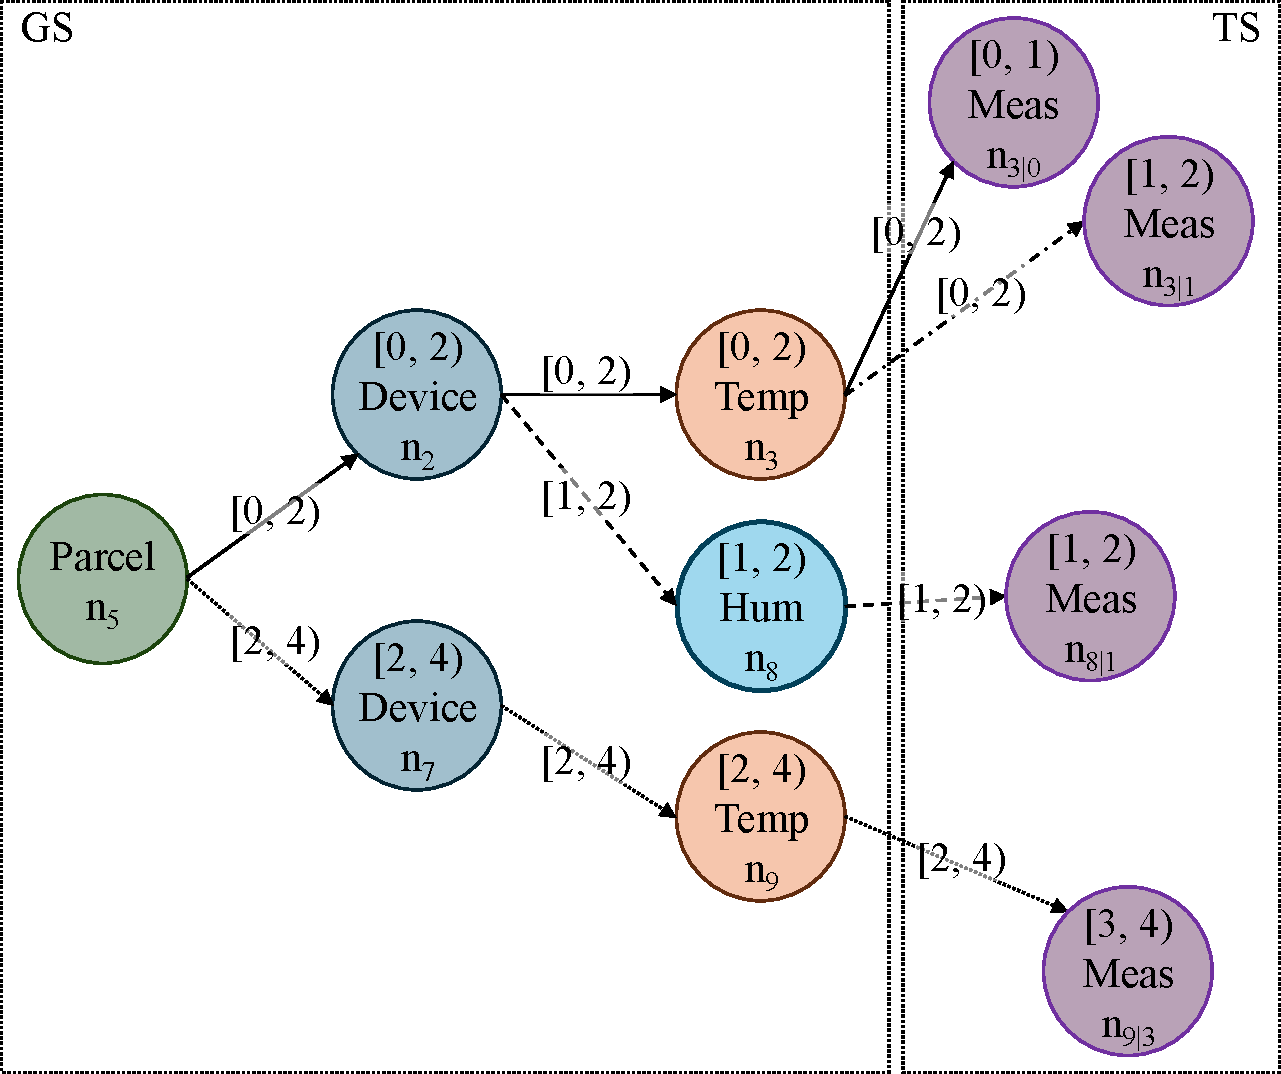
\includegraphics[scale=0.3]{parts/architectures/images/versioning1.pdf}
% \caption{Patterns in the query result with monotonically decreasing temporal validity (from left to right).}\label{fig:versioning1}
% \end{figure}

\begin{example}[Query plan]
In \Cref{fig:example}, $n_2$ was attached to $n_5$ in $[0, 2)$, but then was replaced with $n_7$ in $[2, 4)$.
The Cypher query
\begin{lstlisting}
MATCH (p:Parcel)-[x]->(d:Device)-[y]->(ts)-[z]->(m:Meas)
WHERE p.name = "Parcel 1"
RETURN p, d, ts, m.value
\end{lstlisting}
could have a corresponding query plan $Q$ that is
{\small
\[
\begin{aligned}
R &= \underbrace{\pi_{p,d,ts,m.value}}_{Q[7]}(R_6),&H(R) = (p, d, ts, m.value)\\
R_6 &= \underbrace{\sigma_{m.label = \texttt{Measurement}}}_{Q[6]}(R_5),&H(R_6) = (p, x, d, y, ts, z, m)\\
R_5 &= \underbrace{\varepsilon^{(z,m)}_{ts}}_{Q[5]}(R_4),&H(R_5) = (p, x, d, y, ts, z, m)\\
R_4 &= \underbrace{\varepsilon^{(y,ts)}_d}_{Q[4]}(R_3),&H(R_4) = (p, x, d, y, ts)\\
R_3 &= \underbrace{\sigma_{d.label = \texttt{Device}}}_{Q[3]}(R_2),&H(R_3) = (p, x, d)\\
R_2 &= \underbrace{\varepsilon^{(x,d)}_p}_{Q[2]}(R_1),&H(R_2) = (p, x, d)\\
R_1 &= \underbrace{\sigma_{p.label = \texttt{Parcel}~\land~p.name = ``Parcel~1"}}_{Q[1]}(R_0),&H(R_1) = (p)\\
R_0 &= \underbrace{G^{st}.N}_{Q[0]},&H(R_0) = (p)
\end{aligned}
\]
\noindent where
$R=\begin{array}{|cccc|}
\hline
p & d & ts & m.value \\
\hline
n_5 & n_2 & n_3 & \prop{value}{16} \\
n_5 & n_2 & n_3 & \prop{value}{19} \\
n_5 & n_2 & n_8 & \prop{value}{86} \\
n_5 & n_7 & n_9 & \prop{value}{17} \\
\hline
\end{array}
$, $\ftemporal(t_1)=[0,1), \ftemporal(t_2)=[1,2)$.
}
%\Cref{fig:versioning1} shows the temporal validity (evolving from left to right) of the tuples composing the final relation.
\end{example}

\section{Multistore for graph and time-series}\label{sec:stgraph}

\begin{table}[t]
\centering
\footnotesize
\caption{Data structures of GS and TS. Sizes are in bytes; ``--'' denotes
a variable-size field.}
\label{tbl:structures}
\setlength{\tabcolsep}{4pt}
\begin{tabular}{@{}p{0.23\columnwidth}|
                p{0.23\columnwidth}|
                p{0.23\columnwidth}|
                p{0.23\columnwidth}@{}}
\toprule
\cellcolor{red!20}\textbf{GS Node} &
\cellcolor{blue!20}\textbf{GS Edge} &
\cellcolor{green!20}\textbf{GS Property} &
\cellcolor{orange!20}\textbf{TS Event} \\
\midrule
Id (8)                    & Id (8)                 & Id (8)               & TS id (8) \\
Next property (8)         & Next edge, from (8)    & Next property (8)    & From (8) \\
Next edge (8)             & Next edge, to (8)      & From (8)             & Label (4) \\
From (8)                  & Next property (8)      & To (8)               & Value (8) \\
To (8)                    & From node (8)          & Source id (8)        & Location (--) \\
Label (4)                 & To node (8)            & Source type (1)      & Edges (--) \\
Is TS (1)                 & From (8)               & Type (4)             & Properties (--) \\
                          & To (8)                 & Key (24)             & \\
                          & Label (4)              & Value (8)            & \\
\midrule
\textbf{Total (45)}       &
\textbf{Total (68)}       &
\textbf{Total (77)}       &
\textbf{Total (--)}       \\
\bottomrule
\end{tabular}
\end{table}

\begin{figure}[t]
    \centering
    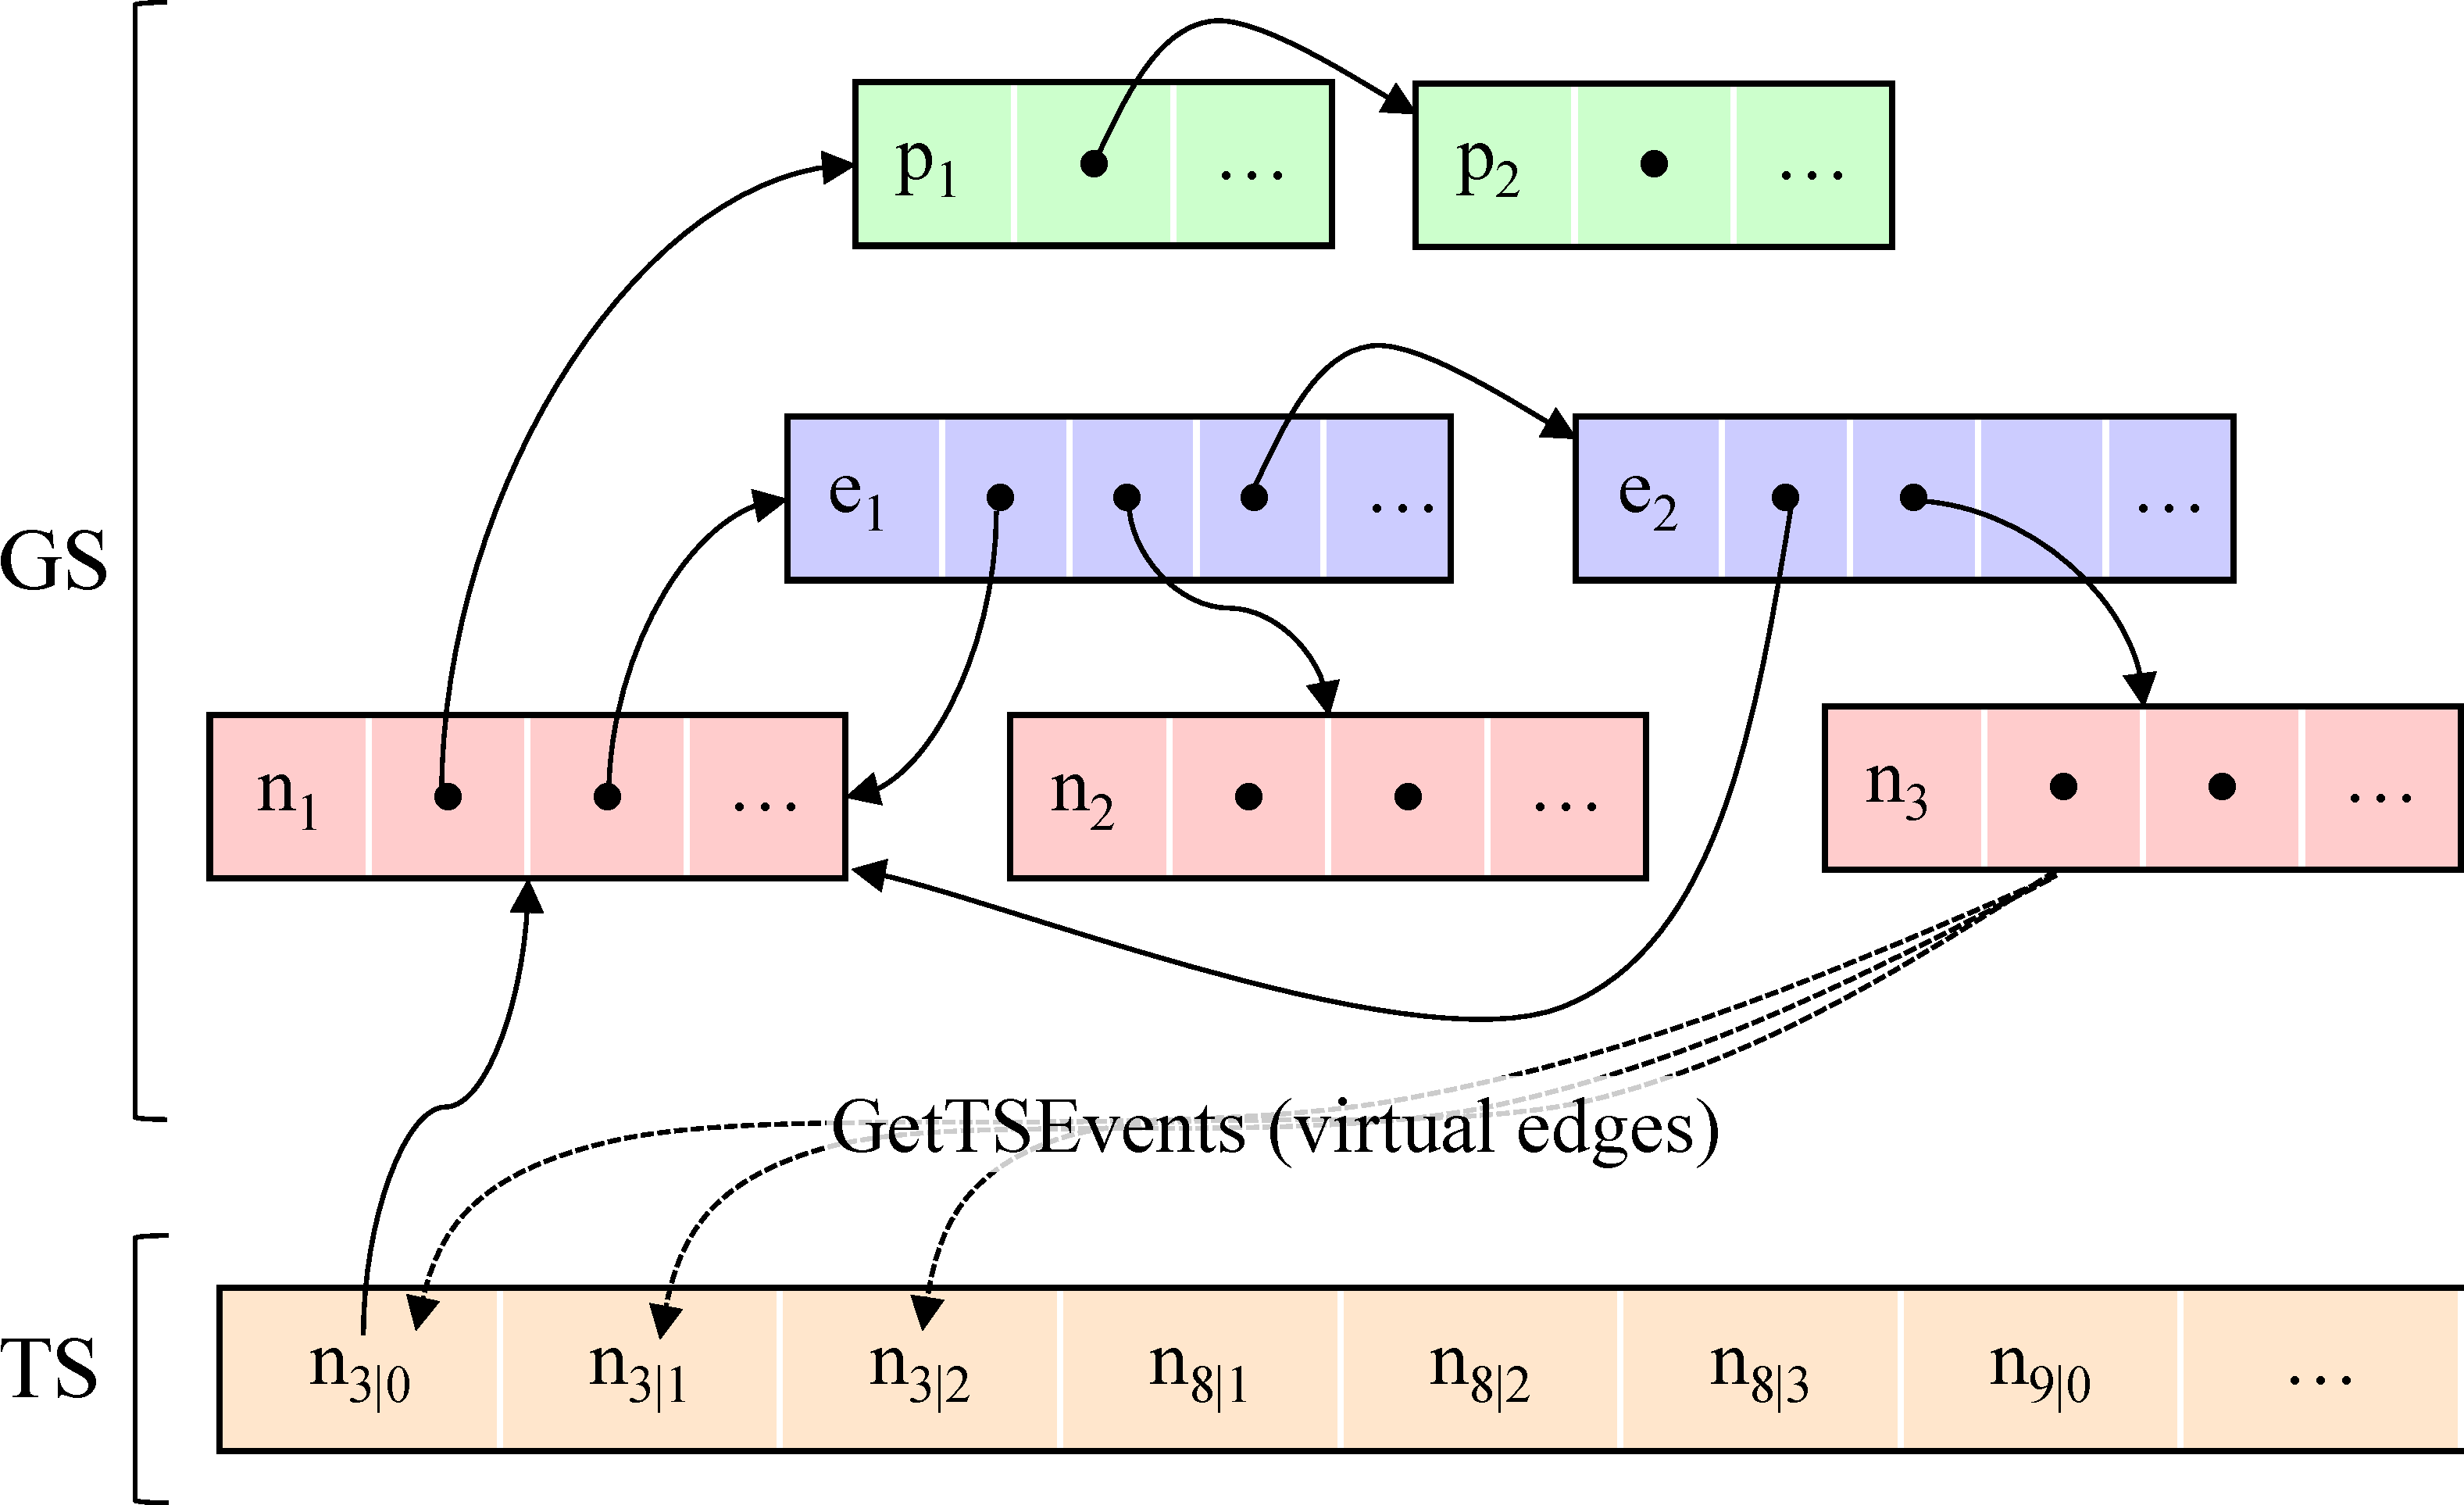
\includegraphics[scale=.145]{parts/architectures/images/overview.pdf}
    \caption{Referring to \Cref{fig:example}, examples of data structures from \Cref{tbl:structures}.
    Events (orange) connected by virtual edges are linked at query time by \textsc{GetTSEvents} in \Cref{alg:search}.}
    \label{fig:structures}
\end{figure}

In \Cref{sec:formal}, we provided \emph{uniform} data and querying abstractions.
From the user's perspective, everything is represented as a spatio-temporal property graph (\Cref{def:stg}).

However, not all graph elements exhibit the same cardinality and access patterns.
Entities such as devices or users are relatively stable and are primarily accessed through graph traversals.
In contrast, temporal events (e.g., measurements) outnumber such entities and are predominantly accessed through temporal filtering, aggregation, and spatial predicates rather than navigation.
Physically storing both using a graph-oriented layout would be suboptimal.%, as graph structures are designed for navigational workloads, whereas event-centric workloads benefit from storage organizations optimized for time-series access.

\subsection{Physical stores}
Following a multistore approach, \ourapproach maps the logical spatio-temporal property graph onto two physical stores.
The Graph Store (GS) persists graph entities and relationships whose primary access pattern is traversal.
The Time-series Store (TS) persists event nodes whose primary access pattern is temporal filtering, aggregation, and spatial lookup.
The two stores are connected through a shared mapping and virtual edges, allowing queries to observe a single spatio-temporal property graph despite the underlying physical separation.
This decoupling allows \ourapproach to inherit the strengths of both physical layouts: it retains structural expressiveness and low-latency graph traversals within GS while ensuring scalable ingestion and querying within TS.
The layouts of the physical stores are summarized in \Cref{tbl:structures} and illustrated in \Cref{fig:structures}.

Referring to \Cref{fig:example}, the logical spatio-temporal property graph includes time-series events as nodes and \lbl{HasEvent} edges. 
% The physical representation (discussed below) preserves this logical abstraction but stores/queries such elements differently.
At query time, time-series events are mapped back to graph nodes, thereby enabling them to hold edges (e.g., $n_{3|0}$ in \Cref{fig:example}) and properties and to serve as traversal points within graph queries.

\subsubsection{Graph Store (GS)}

GS stores nodes, edges, and properties as fixed-size records in independent data structures whose ACID properties are guaranteed through a write-ahead log.
Each GS node stores its temporal validity, a label, a pointer to its first edge, a pointer to its first property, and a flag denoting whether the node owns a time-series in TS (the flag is returned by the function $\fts: N \rightarrow \{true, false\}$).
Each GS edge stores its temporal validity, label, source and destination node identifiers, a pointer to its first property, and next-edge pointers for the adjacency lists of its endpoints.
Each GS property stores its temporal validity, key, value, source identifier, and a next-property pointer.
If the property value fits 8 bytes (e.g., integer, long, or double values or a short UTF-8 String), the value is directly stored in the property.
Otherwise, the value is stored in a key-value Dynamic Store (implemented in RocksDB). % where the key is the ``property id.''

Fixed-size records and pointer chains enable index-free adjacency: traversals follow adjacency lists directly bypassing unrelated records scans or secondary indexes joins.

\subsubsection{Time-series Store (TS)}

%Time-series are long series of events, mostly append-only, and ordered by time.
TS stores all events in a collection distributed on a cluster of machines.
Each event is exposed as a logical graph node, but is physically stored as a variable-size record containing the identifier of its time-series $tsId$, timestamp, label, (nested) properties, (nested) edges, and an optional spatial object.
The primary key of TS collection is $(tsId,timestamp)$, which uniquely identifies an event inside TS.

The collection is indexed by its primary key (and by space through a secondary index) using Log-Structured Merge-tree (LSM-tree) indexes~\cite{DBLP:journals/acta/ONeilCGO96}.
LSM-tree indexes handle highly intensive ingestion workloads efficiently by buffering write operations in memory and periodically flushing them onto disk in batches, making them ideal for continuous ingestion of large volumes of data.

\subsection{Linking and ingesting TS events}
\ourapproach uses a shared mapping to connect GS nodes and TS events.
A GS node or edge identifier $id$ denotes an offset in the corresponding data structure (which stores fixed-size records).
A TS event is addressed by $(tsId,timestamp)$, where $tsId$ identifies the time-series and $timestamp$ identifies the event within that time-series.

Nodes having corresponding time-series in TS are flagged with $\fts(n) = true$ and have a one-to-one mapping with the time-series identifier $tsId$ in TS, i.e., $n.id = tsId$.
This is exploited by the ``Data Collection'' service (\Cref{fig:overview}), enabling each time-series to be continuously ingested independently from GS.
By knowing $tsId$, the decoupled storage allows each event generated by $n$ to be directly appended to the time-series in TS without updating $n$ in GS or materializing a graph edge for each event.
This is how \ourapproach handles high-frequency event streams.
\begin{algorithm}[htp]
\scriptsize
\caption{``Query Service''}
\label{alg:search}
\begin{algorithmic}[1]

\Require Spatio-temporal property graph $G^{st}$, query plan $Q$
\Ensure Relation $R$

\State $R \gets \emptyset$
\label{alg:search:init-result}
\Comment{Result relation}

\State $acc \gets \{(1,(n)) \mid n \in G^{st}.N_{GS}\}$
\label{alg:search:init-acc}
\Comment{Queue accumulator}

\While{$acc$ is not empty}
\label{alg:search:while}
\Comment{Process all pending tuples}

    \State $(i,t) \gets pop(acc)$
    \label{alg:search:pop}

    \item[]
    \Comment{$t$ is the current tuple and $i$ is the index of the operator to be applied to $t$}

    \State $op \gets Q[i]$
    \label{alg:search:get-op}
    \Comment{$op=\varnothing$ if $i \geq |Q|$}

    \Switch{$op$}

        \Case{$\sigma_\theta$}
        \label{alg:search:selection-case}
        \Comment{Selection operator}
            \If{$\sigma_\theta(\{t\}) \ne \varnothing$}
            \label{alg:search:selection-test}
            \Comment{If $t$ satisfies $\theta$}
                \State $acc \gets acc \cup \{(i+1,t)\}$
                \label{alg:search:selection}
            \EndIf
        \EndCase
        
        \Case{$\varepsilon_{a,\theta}^{(x,y)}$}
        \label{alg:search:expand-case}
        \Comment{Expansion operator from node $t[a]$}

            \ForAll{
                $t' \in
                \varepsilon_{a,\theta}^{(x,y)}(\{t\})$
            }
            \label{alg:search:expand-loop}

                \State $acc \gets acc \cup \{(i+1,t')\}$
                \label{alg:search:expand-gs}
                \Comment{Expand edges in GS}

            \EndFor
            \If{$\fts(t[a])$} \Comment{If node $t[a]$ has a corresponding time-series}
                \State $acc \gets acc \cup
                \textsc{QueryTS}(t,a,x,y,i)$
                \label{alg:search:expand-ts}
                \Comment{Expand edges in TS}
            \EndIf

        \EndCase

        \Case{$\pi_A$}
        \label{alg:search:projection-case}
        \Comment{Projection operator}

            \State $acc \gets acc \cup
                \{(i+1,\pi_A(\{t\}))\}$
            \label{alg:search:projection}
            \Comment{Project $t$ and update its schema}

        \EndCase

        \Case{\textbf{default}}
        \label{alg:search:default-case}
        \Comment{No further operator is available}
            \State $R \gets R \cup \{t\}$
            \label{alg:search:result}
            \Comment{Add $t$ to the result relation}
        \EndCase

    \EndSwitch

\EndWhile

\If{$Q[|Q|-1] = \gamma^x_{A,f,a}$}
\label{alg:search:aggregation-test}
\Comment{The last operator is an aggregation}

    \State $R \gets \gamma^x_{A,f,a}(R)$
    \label{alg:search:aggregation}
    \Comment{Group by $A$ and aggregate attribute $a$}

\EndIf

\State \Return $R$
\label{alg:search:return}

\item[]

\Procedure{QueryTS}{$t,a,x,y,i$}
\label{proc:query-push-down}

\Statex \hspace{\algorithmicindent}\textbf{Require:} Tuple $t$, node attr. $a$, edge attr. $x$, event attr. $y$, operator index $i$
\Statex \hspace{\algorithmicindent}\textbf{Ensure:} Tuples extended with virtual edges and time-series events

    \State $n \gets t[a]$
    \label{proc:qpd:get-node}
    \Comment{Retrieve the node bound to attribute $a$}

    \State $acc' \gets \emptyset$
    \label{proc:qpd:init}
    \Comment{Initialize the accumulator}


    \State $\hat{N} \gets \textsc{GetTSEvents}(\{tsId = n.id\}, \varnothing, \varnothing)$
    \label{proc:qpd:query-ts}
    \Comment{Get events from TS}

    \ForAll{$n' \in \hat{N}$}
    \label{proc:qpd:iterate}

        \State $e \gets (n,n')$
        \label{proc:qpd:create-edge}
        \Comment{Construct the virtual edge connecting $n$ and $n'$}

        \State $t' \gets t \cup (e,n')$ \Comment{Extend the tuple, where $H(t')\gets H(t) \cup (x,y)$}
        \label{proc:qpd:extend-tuple}

        \State $acc' \gets acc' \cup \{(i+1,t')\}$
        \label{proc:qpd:add-state}
    \EndFor
    
    \State \Return $acc'$
    \label{proc:qpd:return}

\EndProcedure

\item[]
\Procedure{GetTSEvents}{$\Theta,\Pi,\Gamma$}
\label{proc:query-ts}
\Statex \hspace{\algorithmicindent}\textbf{Require:} Selection predicate $\Theta$, Projection $\Pi$, Aggregation $\Gamma$
\Statex \hspace{\algorithmicindent}\textbf{Ensure:} Events from TS
    \State Implementation of ``Query Rewriter'' (\Cref{fig:overview}), depends on adopted TS engine
\EndProcedure

\end{algorithmic}
\end{algorithm}

\subsection{Querying the spatio-temporal graph}
The seamless querying of GS and TS is carried out by the ``Query Service'' (\Cref{fig:overview} and \Cref{alg:search}).

\Cref{alg:search} describes the execution of a query plan $Q$ over the spatio-temporal property graph $G^{st}$.
The algorithm follows a breadth-first tuple-at-a-time execution based on a queue, denoted by $acc$.
Each element of the queue is a pair $(i,t)$, where $t$ is an intermediate tuple and $i$ identifies the next query operator to be applied to it.
The queue is initialized with one tuple $(n)$ for each node $n \in G^{st}.N_{GS}$\footnote{We start query execution from nodes in GS.}, and each tuple is associated with operator index $1$, since $Q[0]=G^{st}.N_{GS}$ has already produced the initial relation (Line~\ref{alg:search:init-acc}).
Consequently, query evaluation starts independently from every node in the graph.
While the queue is not empty, the algorithm extracts a pair $(i,t)$ (Line~\ref{alg:search:pop}).
It then retrieves the operator $Q[i]$ (Line~\ref{alg:search:get-op}).
If $i \geq |Q|$, no further operator is available and the tuple is considered a final result.
When the current operator is a selection $\sigma_\theta$, the tuple $t$ is evaluated against the predicate $\theta$.
If the predicate is satisfied, the tuple is reinserted into the queue with index $i+1$ (Line~\ref{alg:search:selection}).
Otherwise, the tuple is discarded.
When the current operator is an expansion $\varepsilon_{a,\theta}^{(x,y)}$, the algorithm first evaluates the expansion over GS (each resulting tuple $t'$ is inserted into the queue and associated with the next operator; Line~\ref{alg:search:expand-gs}), then, if the node $t[a]$ has a corresponding time-series, over TS through the $\textsc{QueryTS}$ function; Line~\ref{alg:search:expand-ts}.
The tuples are extended with virtual edges and events are added to the queue.
For a projection operator $\pi_A$, the current tuple is restricted to the attributes in $A$.
The resulting tuple is then associated with index $i+1$ and reinserted into the queue (Line~\ref{alg:search:projection}).
If no operator corresponds to the current index, the tuple has completed the query plan and is inserted into $R$ (Line~\ref{alg:search:result}).
Execution terminates when no additional tuples are in the queue.
Aggregation is handled after all tuples have been collected (Line~\ref{alg:search:aggregation}).
The resulting relation is finally returned (Line~\ref{alg:search:return}).

\paragraph{Traversing time-series nodes}
Since the number of events in TS (e.g., measurements) is significantly higher than the number of nodes in GS (e.g., sensors), physically storing the edges going from GS to TS (\lbl{HasEvent} in \Cref{fig:example}) would require materializing an extremely large number of edges.
%Such a design would not only incur a prohibitive storage overhead but would also negatively impact traversal efficiency.
Instead, we introduce \textit{virtual edges}, i.e. edges that are not physically stored in GS but are generated at query time and returned in the result.

\textsc{QueryTS} (\Cref{alg:search} Line~\ref{proc:query-push-down}) evaluates the expansion towards TS.
%The function receives the current tuple $t$, the id $a$ corresponding to the node from which the expansion starts, the event attribute $y$, and the index $i$ of the current query operator.
First, it retrieves from $t$ the node bound to $a$ (Line~\ref{proc:qpd:get-node}) and initializes an empty set $acc'$ for the tuples produced by the push-down operation (Line~\ref{proc:qpd:init}).
Then, TS is queried using the identifier of $n$ (Line~\ref{proc:qpd:query-ts}).
The query returns a set $\hat{N}$ of events associated with $n$ (i.e., events in TS such that $tsId=n.id$).
For each event $n' \in \hat{N}$, the function constructs a virtual edge $e=(n,n')$ (Line~\ref{proc:qpd:create-edge}) and extends the current tuple $t$ with both the new edge and the event (Line~\ref{proc:qpd:extend-tuple}).
Finally, the function returns all tuples generated through the tuple-store expansion (Line~\ref{proc:qpd:return}).

\paragraph{Traversing events}
Once a TS event is retrieved, it can be traversed by simply filtering its nested edges.

\paragraph{Joining relations}
We do not explicitly incorporate \textsc{Join} into the algorithm since it naturally emerges from the tuple-at-a-time nested-loop evaluation.
In particular, with \Cref{alg:search} we compute the left side of the \textsc{Join}.
For each produced tuple, the same algorithm can then be recursively executed on the right side, using the current tuple as the initial binding.
The tuples returned by the second execution are simply extensions of the original tuple and therefore correspond to the result of a nested-loop join.
Consequently, the \textsc{Join} operator does not require dedicated execution logic and has been omitted from the algorithm for the sake of simplicity.

\section{Query optimization}\label{sec:query}

\begin{figure}[t]
    \centering
    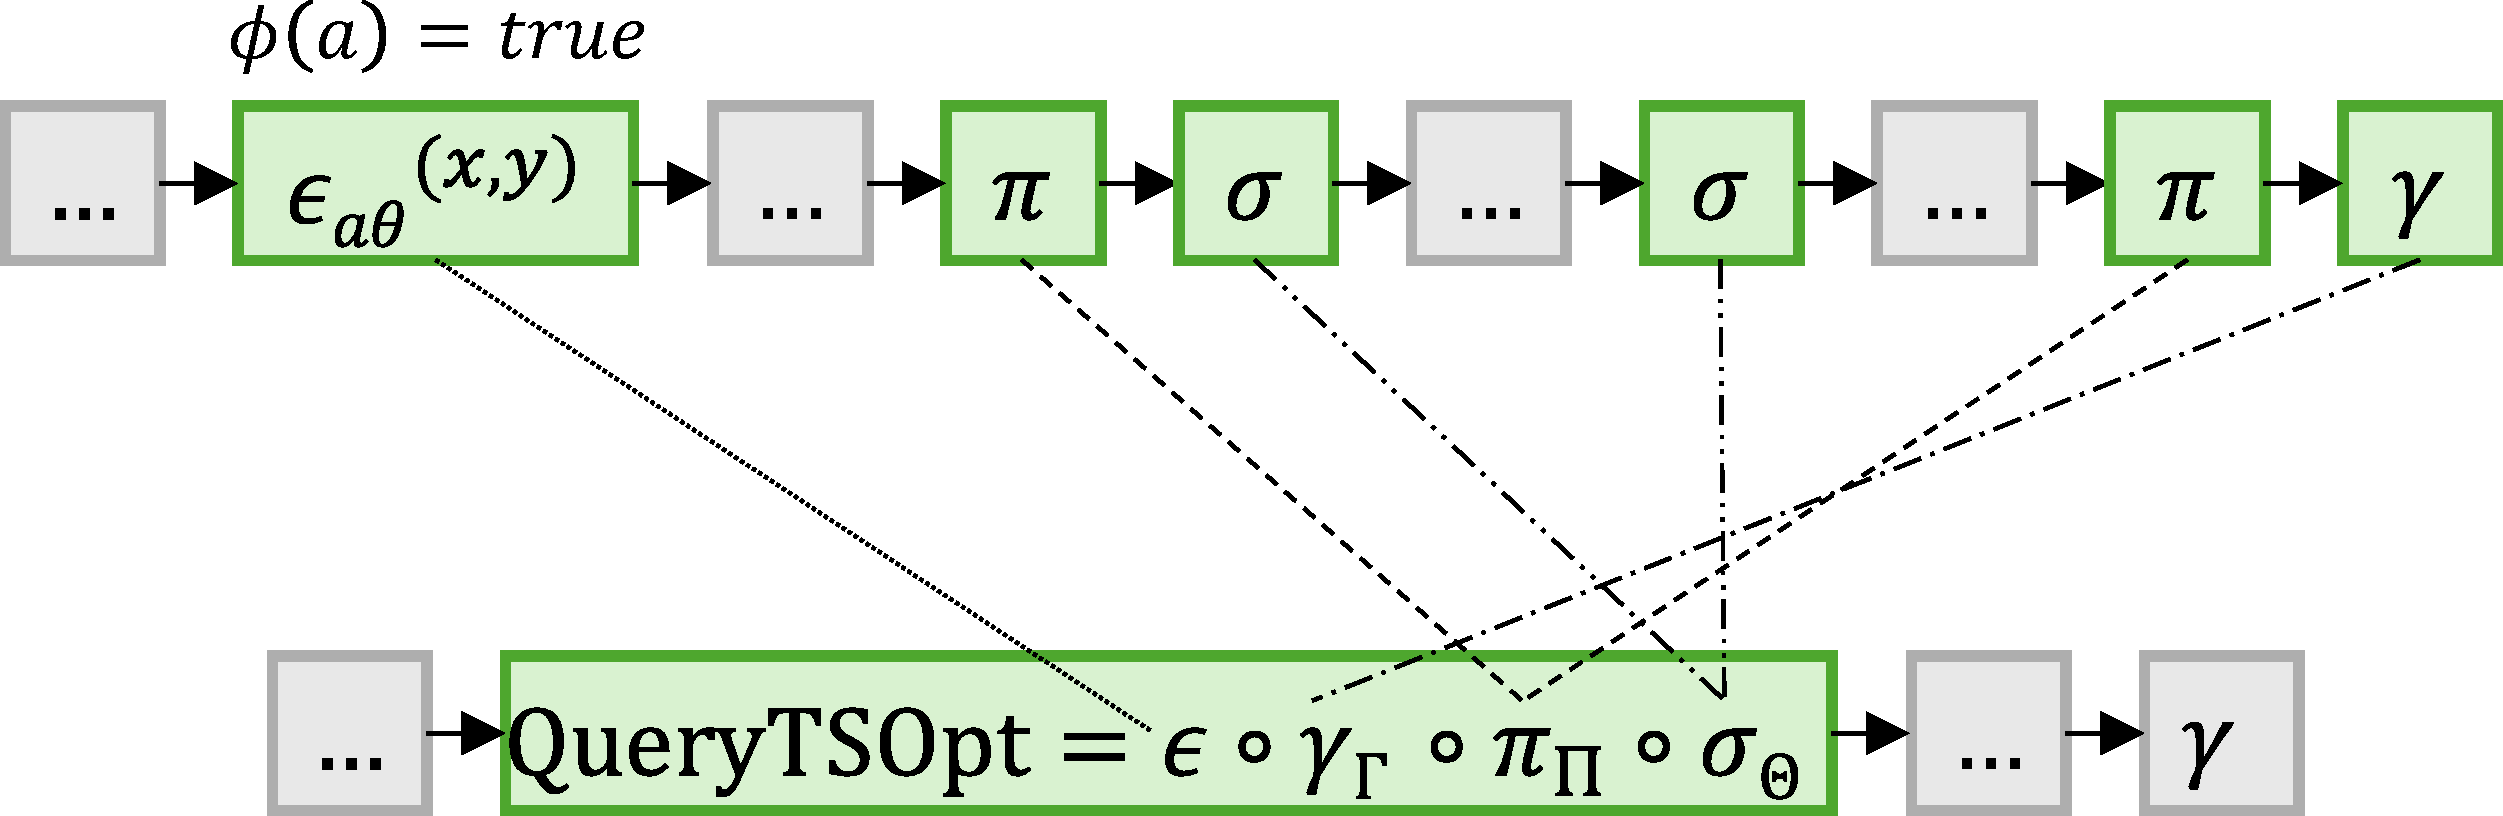
\includegraphics[scale=.18]{parts/architectures/images/opt.pdf}
    \caption{Query optimization to push processing of events down to TS.
    When expanding nodes having corresponding time-series in TS (i.e., $\fts(a)=true$), pushdown is performed by \textsc{QueryTSOpt} (\Cref{alg:query-ts}), which (i) analyzes the query plan to identify predicates, projected properties, and aggregates that depend exclusively on the current time-series variable ($y$), and (ii) fuses and compiles these logical operators into a single physical operator.}
    \label{fig:opt}
\end{figure}

\begin{algorithm}[t]
\footnotesize
\caption{\textsc{QueryTSOpt}}
\label{alg:query-ts}
\begin{algorithmic}[1]

\Require Tuple $t$, node attr. $a$, edge attr. $x$, event attr. $y$, operator idx. $i$, query plan $Q$
\Ensure Tuples extended with virtual edges and time-series events

\Procedure{QueryTSOpt}{$t,a,x,y,i,Q$}
\label{proc:query-ts-opt}

    \State $n \gets t[a]$
    \label{line:qts:get-node}
    \Comment{Retrieve the node bound to $a$}

    \State $acc' \gets \varnothing$
    \label{line:qts:init}
    \Comment{Initialize the result accumulator}

    \State $\Theta \gets \{tsId=n.id\}\cup\textsc{GetPredicates}(t,y,i,Q)$
    \label{line:qts:predicates}
    \Comment{Get the predicates on $y$}

    \State $\Pi \gets \textsc{GetProjectedProperties}(y,i,Q)$
    \label{line:qts:projections}
    \Comment{Get the projections for $y$}

    \State $\Gamma \gets \textsc{GetAggregate}(y,i,Q)$
    \label{line:qts:aggregate}
    \Comment{Get the aggregation by $y$}

    \State $\hat{N} \gets
    \textsc{GetTSEvents}
    \bigl(\Theta,\Pi,\Gamma\bigr)$
    \label{line:qts:query}
    \Comment{Query push down}

    \ForAll{$n' \in \hat{N}$}
    \label{line:qts:iterate}
        \State $e \gets (n,n')$
        \label{line:qts:create-edge}
        \Comment{Construct the virtual edge connecting $n$ and $n'$}
        \State $t' \gets t \cup \{(e,n')\}$
        \label{line:qts:extend}
        \Comment{Extend the tuple, where $H(t')\gets H(t) \cup (x,y)$}
        \State $acc' \gets acc' \cup \{(i+1,t')\}$
        \label{line:qts:accumulate}
    \EndFor
    \State \Return $acc'$
    \label{line:qts:return}
\EndProcedure
\end{algorithmic}
\end{algorithm}

The core contribution of \ourapproach is the transparent cross-store traversal from GS to TS, i.e., the execution boundary where graph traversal expands a node into its associated time-series events.
Consequently, our optimization focuses on this traversal step.
The pushdown towards TS is determined by, and constrained to preserve the semantics of, the portion of the query plan that follows the \textsc{Expand} operator towards time-series events (\Cref{fig:opt}).
Our goal is to find operators in the query plan that can be anticipated and directly computed in TS.
%We optimize the querying of TS when traversing GS nodes.
%As n in \Cref{fig:opt}, our goal is to find operators in the query plan that can be anticipated and directly computed in TS while expanding nodes having a corresponding time-series in TS (i.e., $\fts(a)=true$ in \Cref{fig:opt}).
% When expanding such nodes, 
Pushdown is performed by \textsc{QueryTSOpt} (\Cref{alg:query-ts}) which (i) analyzes the query plan to identify predicates, projected properties, and aggregates that depend on the current time-series variable ($y$), and (ii) fuses and compiles these logical operators into a single physical operator \cite{DBLP:conf/icde/KemperN11,DBLP:conf/cidr/ElgamalLBETRS17} (e.g., logical operators --in green in \Cref{fig:opt}(top)-- are fused into a single physical operator --\Cref{fig:opt}(bottom)).

\textsc{QueryTSOpt} (which replaces \textsc{QueryTS} in \Cref{alg:search}) invokes \textsc{GetPredicates} to construct the set of pushable predicates $\Theta$ (which also includes the predicate $tsId=n.id$; Line~\ref{line:qts:predicates}), \textsc{GetProjectedProperties} (Line~\ref{line:qts:projections}) to determine the set of projected properties $\Pi$, and \textsc{GetAggregate} (Line~\ref{line:qts:aggregate}) to identify an aggregate specification $\Gamma$ that can be delegated to TS.
These operators are compiled together and executed through \textsc{GetTSEvents}.
Consequently, TS returns only the events that satisfy the pushed-down operators.

To simplify the reading of the following algorithms, we will refer to these auxiliary functions.
Given a selection condition $\theta$ (e.g., $\theta = y.val \ge d.thr \land y.ts \ge 10$), $\textsc{Preds}()$ returns the predicates composing the conditions (e.g., $\textsc{Preds}(\theta)=\{y.val \ge d.thr, y.ts \ge 10 \}$) and $\theta$, $\textsc{Operands}()$ returns the single operands (e.g. $\textsc{Operands}(\theta)=\{y.val, d.thr, y.ts\}$ (both excluding constant values).
Given $A \subseteq H(R)$ or a selection condition $\theta$, $\textsc{Attrs}()$ returns the referenced attributes (e.g., $\textsc{Attrs}(\theta)=\{y,d \}$.
Given a single $a \in A$ or operand $p$, $\textsc{Attr}()$ returns the referenced attribute (e.g., $\textsc{Attr}(y.val)=y$).

\subsection{Selection push-down}
\label{subsec:filter-pushdown}

Selection condition can be pushed down to TS to pre-filter events and minimize data shuffling.
A predicate can be pushed to TS only if all of its operands refer to the current time-series (or constants); otherwise, it must be evaluated after the time-series events have been retrieved.
Pushdown is performed by decomposing the selection condition into individual predicates and examining the attributes referenced by each predicate.

\Cref{alg:get-predicates} builds the largest valid predicate $\Theta$ by scanning the suffix of the query plan following $Q[i]$ (Line~\ref{line:gpred:scan}).
Only selection operators are relevant, because they contain predicates that may be evaluated earlier in the plan (Line~\ref{line:gpred:selection}).
A predicate may refer exclusively to $y$ (e.g., $y.ts \ge 10 \land y.ts \le 20$ in green in \Cref{fig:filter-pushdown-example}), or it may also refer to attributes already available in the current tuple (e.g., $y.val \ge d.thr$ in blue in \Cref{fig:filter-pushdown-example}).
The algorithm collects the operands whose attribute is different from $y$ (Line~\ref{line:gpred:external-operands}) since these are external dependencies that prevent the predicate from being directly pushed down.
%The predicate is copied into $pr'$ (Line~\ref{line:gpred:copy}), and each 
Then, each external operand is replaced with its corresponding value from tuple $t$ (Lines~\ref{line:gpred:bind-loop}--\ref{line:gpred:bind}).
For example, given the predicate $y.val \ge d.thr$  and a tuple $t$ such that $t[d].thr = 30$, the binding operation produces $y.val \ge 30$.
The resulting predicate depends only on $y$ and can therefore be pushed down.
%Predicates that already refer only to $y$ have no external operands.
%In that case, the set ($P$) is empty, the binding loop is skipped, and the original predicate is added unchanged to $\Theta$.
%At Line~\ref{line:gpred:add}, each original or bound predicate is inserted into the result set.
Finally, the procedure returns the complete set of pushable predicates at Line~\ref{line:gpred:return}.
A predicate is not pushed down when it does not refer to $y$ or when it refers to another attribute that is not yet present in $H(t)$ (e.g., $y.val \ge z.lim$ in red in \Cref{fig:filter-pushdown-example} since $z$ is introduced by a subsequent expansion and $t[z]$ would be undefined). 

\begin{figure}[t]
\centering
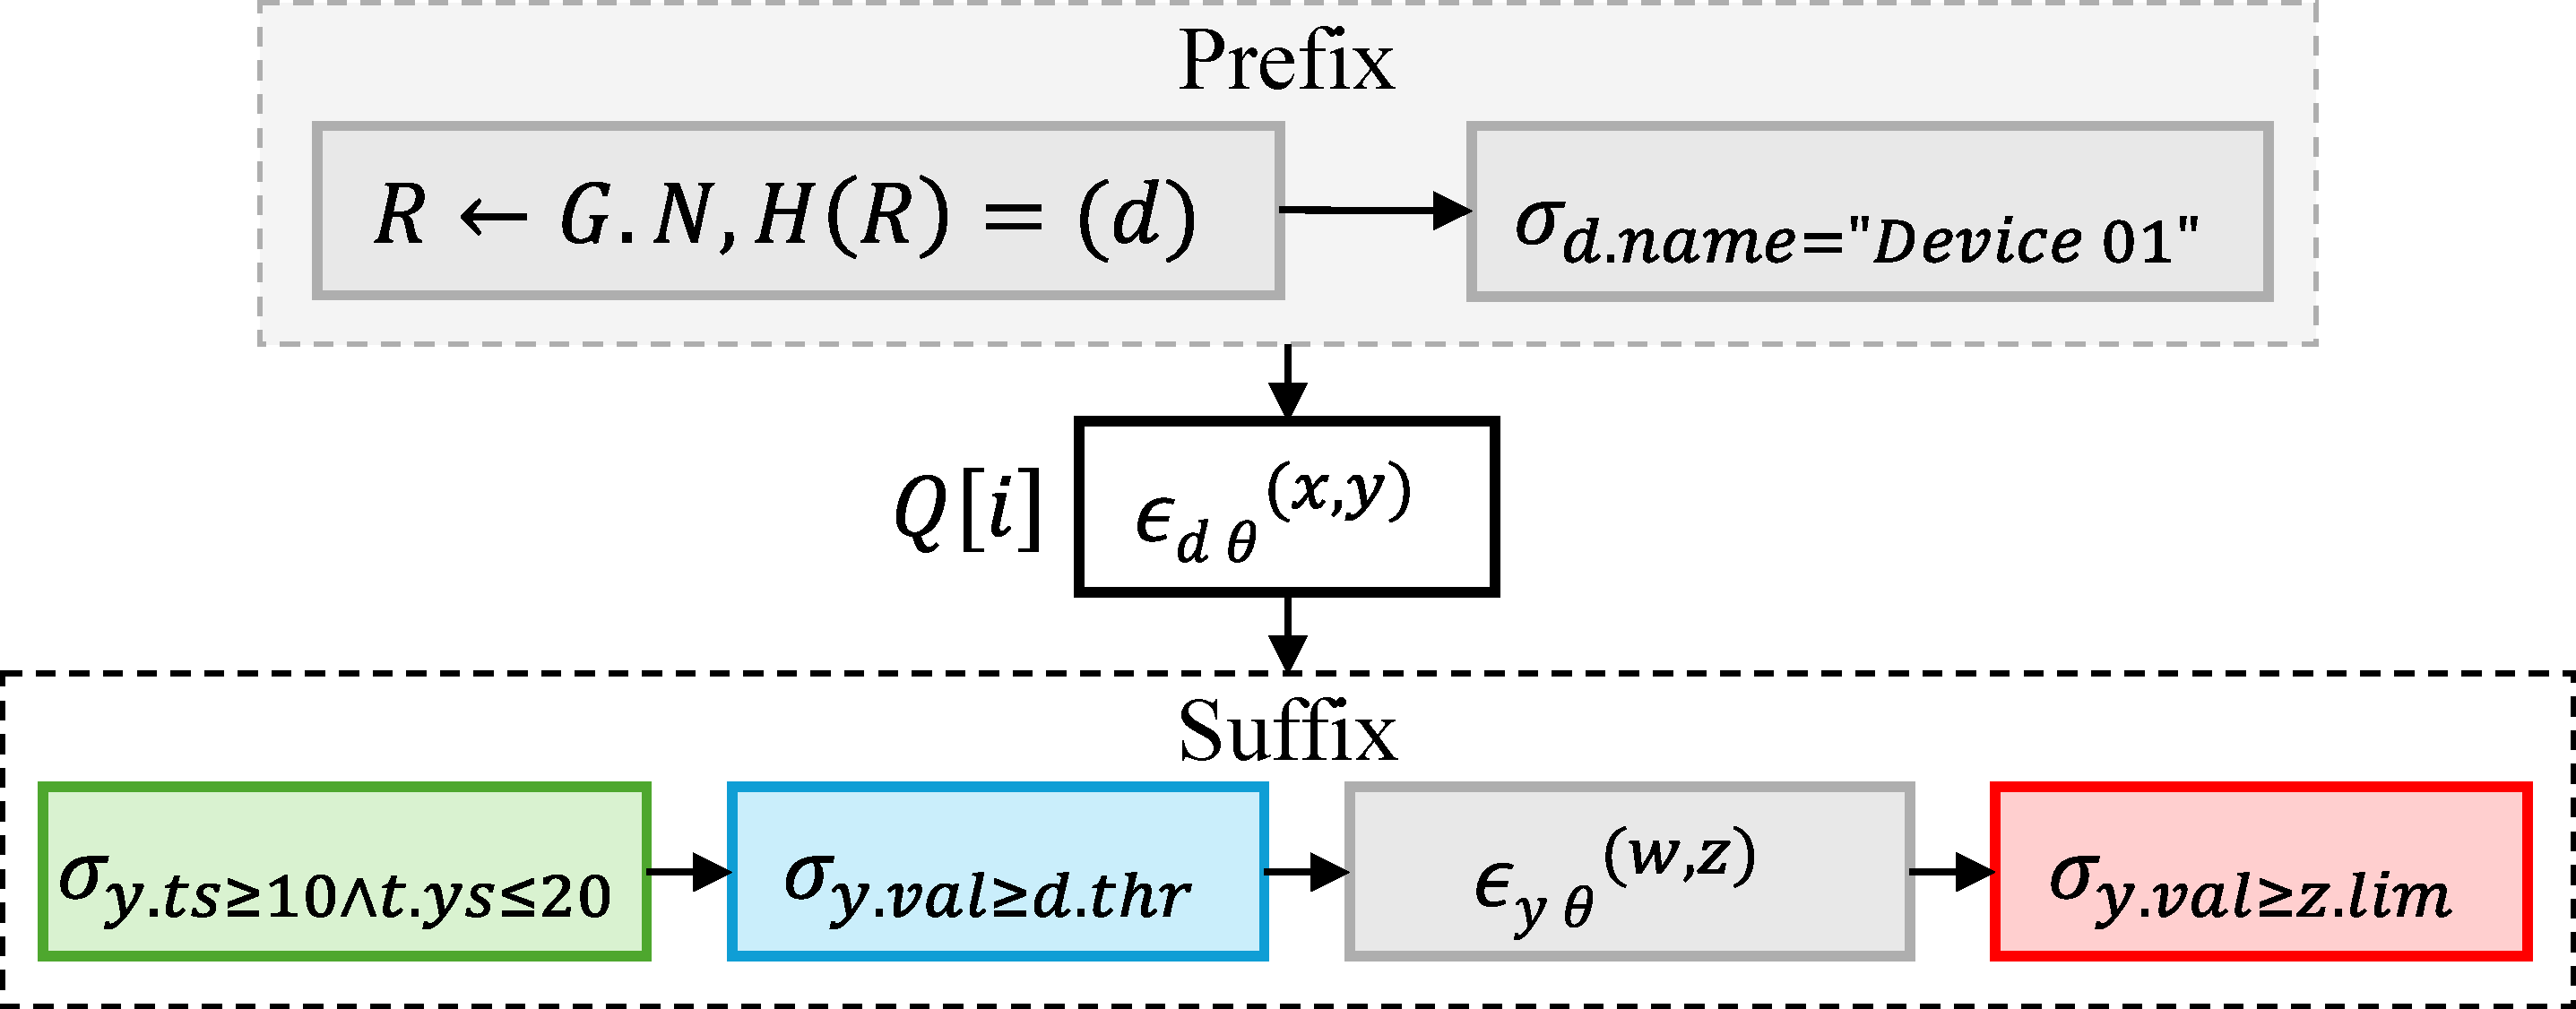
\includegraphics[scale=.165]{parts/architectures/images/filter_pd.pdf}
\caption{
The operator $Q[i]$ expands node $d$ and introduces the edge $x$ and event $y$ attributes.
The predicate $y.ts\ge10\land y.ts\le20$ can be pushed down since it refers only to $y$, while $y.val>d.thr$ can be bound using the value of $d.thr$ since is available when $Q[i]$ is evaluated.
$y.val\ge z.lim$ cannot be pushed down since $z$ is introduced by a subsequent expansion.}
\label{fig:filter-pushdown-example}
\end{figure}

\begin{algorithm}[t]
\scriptsize
\caption{\textsc{GetPredicates}}
\label{alg:get-predicates}
\begin{algorithmic}[1]

\Require Tuple $t$, event attribute $y$, operator index $i$, query plan $Q$
\Ensure Set of predicates $\Theta$

\Procedure{GetPredicates}{$t,y,i,Q$}
    \State $\Theta \gets \varnothing$
    \label{line:gpred:init}
    \Comment{Initialize the set of pushable predicates}

    \For{$op \in Q[i+1:|Q|-1]$}
    \label{line:gpred:scan}
        \Comment{Scan the operators following $Q[i]$}

        \If{$op=\sigma_{\theta}$}
        \label{line:gpred:selection}
            \Comment{Process selection operators only}

            \ForAll{$pr \in \textsc{Preds}(\theta)$}
            \If{$y \in \textsc{Attrs}(pr) \land \bigl(\textsc{Attrs}(pr) \setminus \{y\}\bigr) \subseteq H(t)$}
                \label{line:gpred:predicate-loop}
                \item[]\Comment{Require every attribute other than $y$ to be bound in $t$}
                \State $P \gets
                    \{p \in \textsc{Operands}(pr)
                    \mid \textsc{Attr}(p) \neq y\}$
                \label{line:gpred:external-operands}
                \item[]\Comment{Find operands referring to attributes other than $y$}

                \State $pr' \gets pr$ \Comment{E.g., $pred'\gets y.val \ge d.thr$} 
                \label{line:gpred:copy}

                \ForAll{$p \in P$} 
                \label{line:gpred:bind-loop} \Comment{E.g., $p \gets d.val$}
                    \State $a \gets \textsc{Attr}(p)$ \Comment{E.g., $a\gets d$}
                    \State $k \gets \textsc{Key}(p)$ \Comment{E.g., $k\gets val$}
                    \State $pr' \gets
                        \textsc{Bind}(pr',p,t[a].k)$ {E.g., $pr'\gets y.val \ge 30$}
                    \label{line:gpred:bind}
                    \item[]\Comment{Replace $p$ with its value in the current tuple}
                \EndFor

                \State $\Theta \gets \Theta \cup \{pr'\}$
                \label{line:gpred:add}
                \Comment{Add the predicate}
            \EndIf
            \EndFor
        \EndIf
    \EndFor

    \State \Return $\Theta$
    \label{line:gpred:return}
\EndProcedure

\end{algorithmic}
\end{algorithm}

\subsection{Projection push-down}
\label{subsec:projection-pushdown}

\begin{figure}[t]
    \centering
    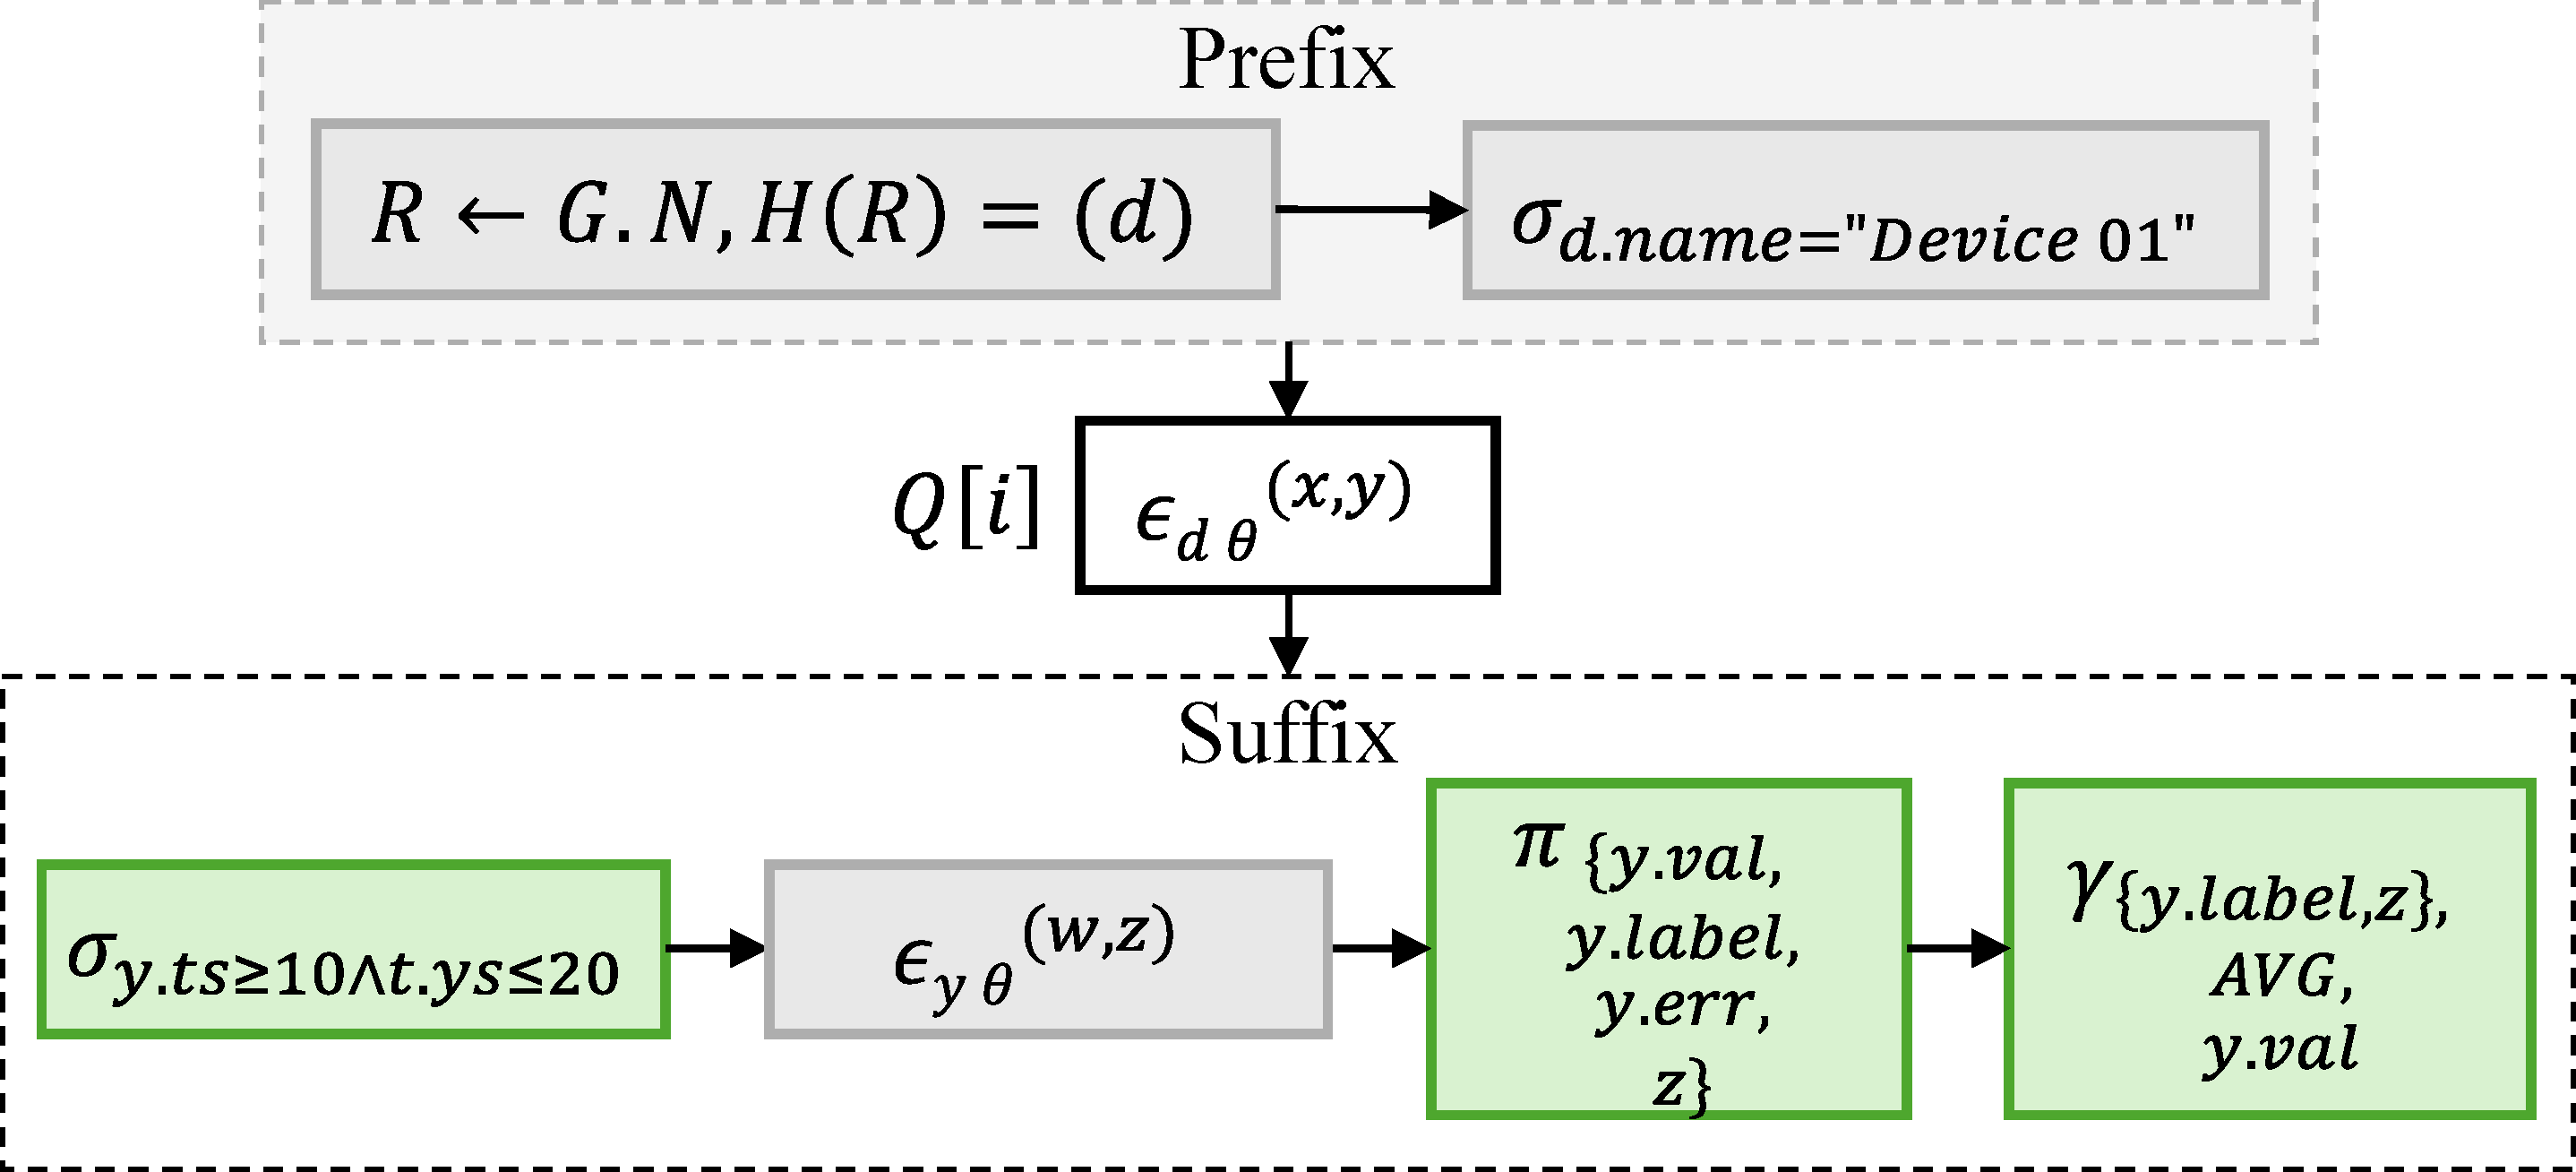
\includegraphics[scale=.165]{parts/architectures/images/projections_pd.pdf}
    \caption{The operator $Q[i]$ expands node $d$ and introduces the edge $x$ and the event $y$ attributes.
    Since the selection, projection, and aggregation requires $y.ts, y.val, y.label, y.err$, only these properties are retrieved for each event in TS.}
    \label{fig:proj-pushdown-example}
\end{figure}

\begin{algorithm}[t]
\scriptsize
\caption{\textsc{GetProjectedProperties}}
\label{alg:get-projections}
\begin{algorithmic}[1]

\Require Event attribute $y$, operator index $i$, query plan $Q$
\Ensure Set of projected properties $\Pi$

\Procedure{GetProjectedProperties}{$y,i,Q$}
\label{proc:get-projections}
    \State $\Pi \gets \emptyset$
    \label{line:gproj:init}
    \Comment{Initialize the set of required properties}
    \ForAll{$op \in Q[i+1:|Q|-1]$}
    \label{line:gproj:scan}
    \Comment{Inspect every operator in the query plan}
        \Switch{$op$}
            \Case{$\pi_A$}
            \label{line:gproj:projection-case}
            \Comment{Process a projection operator}
                \ForAll{$p \in A ~\textbf{s.t.}~ y = \textsc{Attr}(p)$}
                \label{line:gproj:projection-terms}
                \Comment{Properties of $y$}
                    \State $\Pi \gets \Pi \cup \{p\}$
                    \label{line:gproj:add-projection}
                    \Comment{Record the projected property}
                \EndFor
            \EndCase
            \Case{$\sigma_\theta$}
            \label{line:gproj:selection-case}
            \Comment{Process a selection predicate}
                \ForAll{
                    $p \in \textsc{Operands}(\theta)
                    ~\textbf{s.t.}~
                    y = \textsc{Attr}(p)$
                }
                \label{line:gproj:selection-operands}
                \Comment{Operands of $y$}
                    \State $\Pi \gets \Pi \cup \{p\}$
                    \label{line:gproj:add-selection}
                    \Comment{Record the property used by the predicate}
                \EndFor
            \EndCase 
            \Case{$\gamma^x_{A,f,a}$}
            \label{line:gproj:aggregation-case}
            \Comment{Process an aggregation operator}
                \ForAll{$p \in (A \cup \{a\}) ~\textbf{s.t.}~ y = \textsc{Attr}(p)$}
                \label{line:gproj:grouping-terms}
                \Comment{Grouping of $y$}
                    \State $\Pi \gets \Pi \cup \{p\}$
                    \label{line:gproj:add-grouping}
                    \Comment{Record the properties used by aggregation}
                \EndFor
                % \If{$y = \textsc{Attr}(a)$}
                % \label{line:gproj:aggregate-test}
                % \Comment{Check if the aggregation belongs to $y$}
                %     \State $\Pi \gets \Pi \cup \{a\}$
                %     \label{line:gproj:add-aggregate}
                %     \Comment{Record the aggregate argument}
                % \EndIf
            \EndCase
        \EndSwitch
    \EndFor

    \State \Return $\Pi$
    \label{line:gproj:return}
    \Comment{Return all properties of $y$ required to evaluate $Q$}
\EndProcedure

\end{algorithmic}
\end{algorithm}
Projection push-down anticipates the projection to TS to reduce the amount of data transferred across the two stores.
Only the properties required by operators that cannot be pushed down need to be retrieved from TS.
%The set of projected time-series properties is determined by the remaining portion of the query plan: only the properties required by operators that cannot be pushed down need to be retrieved from TS.

\Cref{alg:get-projections} determines which properties must be retrieved by scanning the suffix of the query plan following $Q[i]$ (Line~\ref{line:gproj:scan}).
For a projection operator $\pi_A$, the function examines the projected terms in $A$ (Line~\ref{line:gproj:projection-case}).
Every term $p$ whose attribute refer to $y$ is inserted into $\Pi$ (Line~\ref{line:gproj:add-projection}; e.g., $y.val, y.err, y.label$ in \Cref{fig:proj-pushdown-example}).
% These properties are required because they must be included in the output tuples produced by the projection. 
For a selection operator $\sigma_\theta$, the function examines the operands of $\theta$ (Line~\ref{line:gproj:selection-case}).
An operand is added to $\Pi$ when it references attribute $y$ (Line~\ref{line:gproj:add-selection}).
Such properties must be available to evaluate the corresponding predicates (e.g., $y.ts$ in \Cref{fig:proj-pushdown-example}).
For an aggregation operator $\gamma^x_{A,f,a}$, the function inspects the grouping terms (Line~\ref{line:gproj:aggregation-case}) and those associated with $y$ are added to $\Pi$ (Line~\ref{line:gproj:add-grouping}; e.g., $y.label$ and $y.val$ in \Cref{fig:proj-pushdown-example}).
% The aggregate argument $a$ is then examined separately in Line~\ref{line:gproj:aggregate-test}.
% If it refers to $y$, it is inserted into $\Pi$ in Line~\ref{line:gproj:add-aggregate}, since its value is required to compute the aggregation function $f$ (e.g., $y.val$ in \Cref{fig:proj-pushdown-example}).

\subsection{Aggregate push-down}
\label{subsec:aggregate-pushdown}

\begin{algorithm}[t]
\footnotesize
\caption{\textsc{GetAggregate}}
\label{alg:get-aggregate}
\begin{algorithmic}[1]

\Require Event attribute $y$, operator index $i$, query plan $Q$
\Ensure Aggregate specification $\Gamma$

\Procedure{GetAggregate}{$y,i,Q$}
\label{proc:get-aggregate}
    \State $\Gamma \gets \varnothing$
    \If{$\not\exists op \in Q[i+1:|Q|-1]~\textbf{s.t.}~op=\varepsilon^{w,z}_{a,\theta} \land a = y$}\label{line:ga:expand-check}
        \item[]\Comment{No further expand on $y$} 

        \For{$op \in Q[i+1: |Q| - 1]$}

        \If{$op=\gamma_{A,f,a}^w \land f\textup{ is not holistic } \land y = \textsc{Attr}(a)$}\label{line:ga:aggregate-check}\Comment{Aggregate $y$} 
            \State $\Gamma \gets
            \left(
                \{p \in A \mid y = \textsc{Attr}(p)\},
                f,
                a
            \right)$
            \label{line:ga:construct}
            \Comment{Aggregate specification}
        \EndIf
        \EndFor
    \EndIf
    \State \Return $\Gamma$
    \label{line:ga:return-empty}
\EndProcedure
\end{algorithmic}
\end{algorithm}
If possible, aggregation push-down anticipates the execution of aggregation operators in TS, thereby reducing the amount of data transferred and exploiting the superior efficiency of TS for aggregating large collections of events.
An aggregation can be delegated when its aggregate argument depends on the current time-series.
As a result, TS returns aggregated values instead of raw events, substantially reducing both data transfer and processing by the query engine.
For distributive aggregation functions (e.g., $\{\mathrm{COUNT}, \mathrm{SUM}, \mathrm{MIN}, \mathrm{MAX}\}$), \textsc{GetTSEvents} computes partial aggregates over TS and \Cref{alg:search} later combines these partial results to obtain the final global aggregate.
Since distributive functions are associative and composable, this optimization preserves the exact query semantics while significantly reducing the amount of data transferred between the two stores.
Algebraic aggregation functions, such as $\mathrm{AVG}$, are handled by computing the corresponding partial aggregates in TS (e.g.,  $\{\mathrm{COUNT}, \mathrm{SUM}\}$) and eventually combining them to derive the final result.
Holistic aggregation functions (e.g., $\mathrm{MEDIAN}$) cannot be decomposed into independent partial aggregates.

\Cref{alg:get-aggregate} identifies whether an aggregation involving the event attribute $y$ can be pushed down.
% The function \textsc{GetAggregate}, identified by \Cref{proc:get-aggregate}, receives the event attribute $y$, the index $i$ of the current operator, and the query plan $Q$.
The function verifies that the portion of the query plan following position $i$ does not contain an expansion operator whose source attribute is $y$ (Line~\ref{line:ga:expand-check}).
A subsequent expansion from $y$ requires the original event instances to remain available; therefore, aggregating them in advance could discard information required by the expansion.
If no such expansion exists, the function scans the operators occurring after position $i$.
For each operator, it checks whether the operator is a not-holistic aggregation $\gamma^w_{A,f,a}$ where $a$ belongs to event attribute $y$ (Line~\ref{line:ga:aggregate-check}; e.g., $\gamma_{\{y.label,z\},\mathrm{AVG},y.val}$ in \Cref{fig:proj-pushdown-example}).
If so, the function constructs the aggregate specification $\Gamma$ (Line~\ref{line:ga:construct}), where the first component contains the grouping properties in $A$ associated with $y$ (e.g., $\{y.label\}$), $f$ is the aggregation function, and $a$ is the property over which the aggregation is evaluated (e.g., $y.val$).
Grouping attributes not associated with $y$ (e.g., $z$) are eventually considered when combining the partial aggregates.

\subsection{Multi-threaded query execution}
\label{subsec:query-parallel-execution}

For both \textsc{QueryTS} and \textsc{QueryTSOpt}, the invocation of \textsc{GetTSEvents} can be executed concurrently since the TS requests are independent for each tuple.
% For instance, in \textsc{QueryTSOpt} (\Cref{alg:query-ts}), each invocation retrieves the node bound in its own tuple at Line~\ref{line:qts:get-node} and independently constructs its filter, projection, and aggregate specifications at Lines~\ref{line:qts:predicates}--\ref{line:qts:aggregate}.
% Once these parameters have been derived, the request issued at Line~\ref{line:qts:query} depends only on the bindings contained in the corresponding tuple and does not depend on the results of requests generated for other tuples.
Given an input relation
$
    R=\{t_i,\ldots\},
$
the ``Query Service'' can generate one request 
$
    \textsc{GetTSEvents}
    \bigl(
        \Theta_i,
        \Pi_i,
        \Gamma_i
    \bigr)$
for each tuple $t_i$
.
This independence enables a multi-threaded execution in which the requests are submitted to a pool of worker threads.
Each worker sends one request to TS and processes the returned events by performing the tuple-extension operations.

Parallel execution is effective when time-series retrieval is I/O-bound or when TS supports concurrent requests, since latency is determined by the slowest batch rather than by the sum of all requests.
The degree of parallelism must be bounded to avoid overloading TS or exhausting network connections.
Our implementation uses a fixed-size thread pool, sized according to the resources of the ``Query Service'' and the concurrency supported by TS, whose workers update a thread-safe shared accumulator.

\section{Experimental evaluation}\label{sec:exp}

\begin{table}[t]
\centering
\footnotesize
\caption{Dataset statistics.}
\label{tab:datasets}
\begin{tabular}{lcccc}
\toprule
Dataset       & Size & Nodes & Edges & Avg.
TS events\\
\midrule
\multirow{3}{*}{\textsf{MIV}} & S    & $1.7 \cdot 10^6$   & $1.7 \cdot 10^6$ & $2.5 \cdot 10^3$ \\
              & M    & $1.7 \cdot 10^7$   & $1.7 \cdot 10^7$ & $2.5 \cdot 10^3$ \\
              & L    & $1.7 \cdot 10^8$   & $1.7 \cdot 10^8$ & $2.6\cdot10^3$ \\\midrule
\multirow{3}{*}{\textsf{SB}}  
              & S    & $2.5\cdot10^{6}$   & $2.5\cdot10^{6}$ & $2.5\cdot10^{4}$ \\
              & M    & $1.0\cdot10^{7}$   & $1.0\cdot10^{7}$ & $5.1\cdot10^{4}$ \\
              & L    & $2.6\cdot10^{8}$   & $2.6\cdot10^{8}$ & $2.5\cdot10^{5}$ \\
              & XL   & $3.0\cdot10^{8}$   & $3.0\cdot10^{8}$ & $1.5\cdot10^{6}$ \\
\bottomrule
\end{tabular}

%\begin{table}[t]
%\centering
%\footnotesize
\caption{Characteristics of query workload.}
\label{tab:queries}
\begin{tabular}{lcccccccc}
\toprule
           &    & \multicolumn{2}{c}{Store} & \multicolumn{5}{c}{Operators}\\
           \cmidrule(lr){3-4}\cmidrule(lr){5-9}
Dataset  & ID & GS        & TS          & Join                & Aggregate     & Select    & Expand        & Project   \\\midrule
\multirow{3}{*}{\textsf{SB}}& Q1 & \ding{51} &             &                     &               & \ding{51} & \ding{51}     & \ding{51} \\
           & Q2 & \ding{51} & \ding{51}   & \ding{51}           & \ding{51}     & \ding{51} & \ding{51}     & \ding{51} \\
           & Q3 & \ding{51} & \ding{51}   & \ding{51}           &               & \ding{51} & \ding{51}     & \ding{51} \\
           & Q4 & \ding{51} & \ding{51}   & (spatial)           & \ding{51}     & \ding{51} & \ding{51}     & \ding{51} \\
           & Q5 & \ding{51} & \ding{51}   &                     & \ding{51}     & \ding{51} & \ding{51}     & \ding{51} \\
           & Q6 & \ding{51} &             &                     & \ding{51}     & \ding{51} & \ding{51}     & \ding{51} \\\midrule
\multirow{3}{*}{\textsf{MIV}}  & Q1 & \ding{51} &             &                     &               & \ding{51} & \ding{51}     & \ding{51} \\
           & Q2 & \ding{51} & \ding{51}   &                     & \ding{51}     &           & \ding{51}     & \ding{51} \\
           & Q3 & \ding{51} & \ding{51}   &                     & \ding{51}     & \ding{51} & \ding{51}     & \ding{51} \\
\bottomrule
\end{tabular}
\end{table}

The implementation and evaluation of \ourapproach is available at \url{https://github.com/big-unibo/stgraph}.
GS is centralized and runs on a single machine, while TS is distributed across multiple machines in a cluster.
GS has been developed in Kotlin and TS has been implemented in AsterixDB~\cite{DBLP:journals/pvldb/AlsubaieeAABBBCCCFGGHKLLOOPTVWW14}.
Time-series are stored as an AsterixDB dataset of records partitioned across nodes in a cluster and indexed through LSM-tree indexes~\cite{DBLP:journals/pvldb/AlsubaieeBBHKCDL14}.
AsterixDB also supports secondary indexes, including a spatial LSM R-tree~\cite{DBLP:journals/pvldb/AlsubaieeBBHKCDL14} used to index the \texttt{location} property and Data Feeds~\cite{DBLP:conf/edbt/GroverC15} to implement high-throughput ingestion adapters for time-series data.
%
% A Data Feed allows the definition of an ingestion pipeline that maps incoming data from an external source (operating in either push or pull mode) directly into existing datasets.
%
% \ourapproach assigns a dedicated data feed to each time-series node, enabling parallel streaming ingestion across multiple data sources.
%
The storage replication factor in AsterixDB was fixed to 1 to take into account raw storage costs only.

Experiments were conducted on a cluster of machines equipped with an Intel Xeon W5-2445 processor (20 cores, 4.6 GHz) and 256 GB of DDR5 RAM.
%In the following, we first describe the datasets and queries used for testing, and then we present the results of the evaluation.

\subsection{Datasets}

For the testing datasets, \Cref{tab:datasets} summarizes the number of nodes and edges and the average time-series length. 
Overall, (1) \textsf{MIV} contains thousands of shorter time-series (up to $2.6 \cdot 10^3$ events on average), while \textsf{SB} contains fewer but longer time-series (up to $1.5\cdot10^6$ events on average), and (2) the number of time-series events is orders of magnitude higher than the volume of master data, which motivates the need for a hybrid data structure and optimized query execution.

\subsubsection{Medical Information Mart for Intensive Care IV (\textsf{MIV})}

\textsf{MIV} \cite{johnson2020mimic} is a large deidentified dataset of patients admitted to the emergency department or an intensive care unit.
It contains data for patients admitted to an ICU and incorporates health-care time-series data.
Large is the full version of the dataset, while Small ($\times\frac{1}{100}$) and Medium ($\times\frac{1}{10}$) are downscaled versions.
Mimic queries range over the whole graph.
Q1 filters on healthcare events.
Q2 computes the average values of all time-series.
Q3 combines Q1 and Q2 by averaging values of filtered time-series. 

\subsubsection{SmartBench (\textsf{SB})}
\textsf{SB}~\cite{DBLP:journals/pvldb/GuptaCMY20} is a benchmark derived from a real-world smart building monitoring system.
It models devices composed of sensors performing high-frequency measurements and the spatial structure of the monitored environment.
\textsf{SB} provides a tool to generate datasets of increasing scaling factors: Small ($\times1$), Medium ($\times4$), and Large ($\times100$); XL is a variation of M with artificially-extended time-series.

\textsf{SB} also defines queries that differ in terms of filtering conditions, aggregation functions, and selection criteria.
The characteristics of the queries selected for evaluation are detailed in \Cref{tab:queries} (the complete specification of the queries can be found in \cite{DBLP:journals/pvldb/GuptaCMY20}).
Q1 is a graph traversal query that does not require access to TS.
Q2 and Q5 are analytical queries; Q2 has a high-selectivity filter (it includes $\approx12\%$ events), while Q5 has a low-selectivity filter (it includes $\approx37\%$ of events).
Q3 and Q4 join graph nodes and time-series events based on existence conditions on specific events.
Q4 involves a spatial join operation, since a device may produce data within an environment without being explicitly connected to it through a graph edge. 
Finally, Q6 gets all the historical relationships of a sensor, including all past measurements.

\subsection{Pushdown: \textsc{QueryTS} vs \textsc{QueryTSOpt}}

\Cref{fig:opt_vs_naive} and \Cref{tbl:opt_vs_naive} compare the performance of \textsc{QueryTS} and \textsc{QueryTSOpt} (see \Cref{sec:query}); intuitively, \textsc{QueryTS} collects all data before processing it, while \textsc{QueryTSOpt} pushes event processing down to TS.
GS and TS run on the same machine and use 1 thread.

\textsc{QueryTSOpt} consistently outperforms \textsc{QueryTS}.
For the \textsf{MIV} dataset, execution times are reduced by approximately one order of magnitude, while on the more demanding \textsf{SB} workload the gains are even larger, reaching or exceeding two orders of magnitude for the most time-series-intensive queries (Q1 in \textsf{SB} is not affected by the optimization since it only involves operations on GS). 
Moreover, \textsc{QueryTS} does not complete within practical limits (marked as \oot) for several query-dataset combinations.
The benefits of \textsc{QueryTSOpt} become more pronounced as time-series length and data scan increase (e.g., less selective predicates or group by on the whole time-series), confirming the effectiveness of the proposed optimizations.
This is particularly evident in \textsf{SB} Q3 that must verify whether each time-series satisfies a given condition (e.g., contains at least one measurement above a threshold).
While \textsc{QueryTS} shuffles all data back to GS, \textsc{QueryTSOpt} directly checks the time-series in TS and only returns the relevant information, resulting in speedups of orders of magnitude.

\begin{figure}[t]
    \centering
    \begin{subfigure}[t]{\columnwidth}
        \centering
        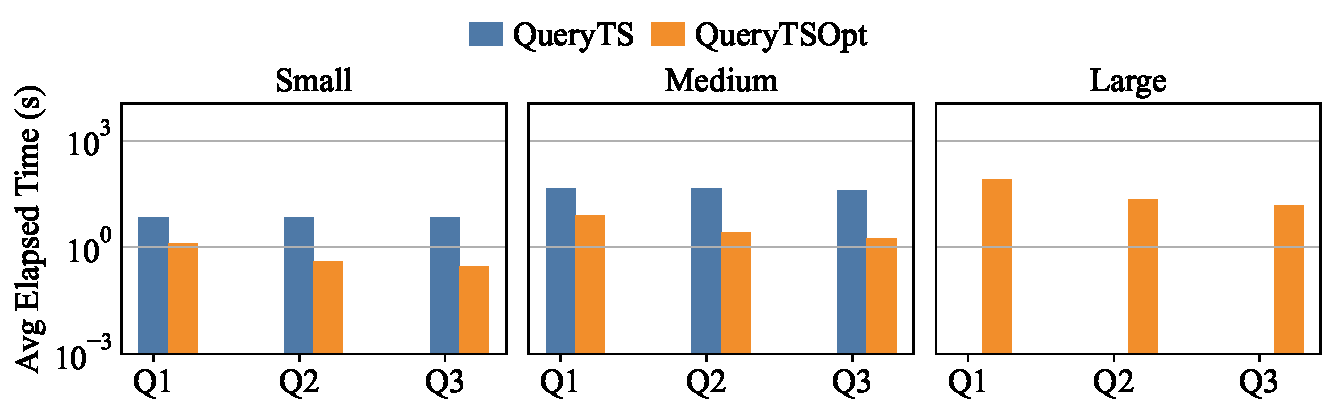
\includegraphics[scale=.6]{parts/architectures/images/query_opt_mimic.pdf}
        \caption{\textsf{MIV}}
    \end{subfigure}
    \begin{subfigure}[t]{\columnwidth}
        \centering
        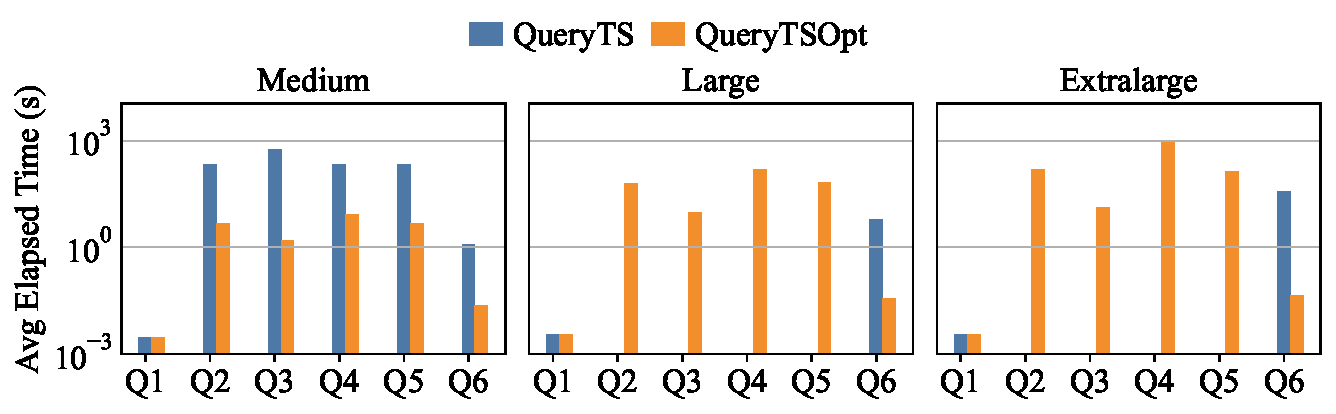
\includegraphics[scale=.6]{parts/architectures/images/query_opt_smartbench.pdf}
        \caption{\textsf{SB}}
    \end{subfigure}
    \caption{\textsc{QueryTS} vs \textsc{QueryTSOpt}.
For both \textsf{SB} and \textsf{MIV}, \textsc{QueryTS} fails to compute for queries accessing too much data.
For the sake of space, \textsf{SB}-Small has been omitted.
}
\label{fig:opt_vs_naive}
\end{figure}

\begin{table}[t]
\centering\footnotesize
\caption{\textsc{QueryTS} vs \textsc{QueryTSOpt}.}
\label{tbl:opt_vs_naive}
\setlength{\tabcolsep}{2.5pt}
\renewcommand{\arraystretch}{0.9}
\resizebox{\columnwidth}{!}{%
\begin{tabular}{lcccccccc}
\toprule
 &  & & Q1 & Q2 & Q3 & Q4 & Q5 & Q6 \\
Dataset & Size & Mode &  &  &  &  &  &  \\
\midrule
\multirow[*]{5}{*}{\textsf{MIV}} & \multirow[*]{2}{*}{S} & \textsc{QueryTS} & $6.8 \cdot 10^{0}$ & $7.1 \cdot 10^{0}$ & $7.2 \cdot 10^{0}$ & -- & -- & -- \\
 &  & \textsc{QueryTSOpt} & $1.3 \cdot 10^{0}$ & $4.0 \cdot 10^{-1}$ & $3.0 \cdot 10^{-1}$ & -- & -- & -- \\
\cline{2-9}
 & \multirow[*]{2}{*}{M} & \textsc{QueryTS} & $4.7 \cdot 10^{1}$ & $4.6 \cdot 10^{1}$ & $3.9 \cdot 10^{1}$ & -- & -- & -- \\
 &  & \textsc{QueryTSOpt} & $7.9 \cdot 10^{0}$ & $2.6 \cdot 10^{0}$ & $1.8 \cdot 10^{0}$ & -- & -- & -- \\
\cline{2-9} & \multirow[*]{2}{*}{L} & \textsc{QueryTS} & \oot & \oot & \oot & -- & -- & -- \\
 &  & \textsc{QueryTSOpt} & $7.9 \cdot 10^{1}$ & $2.2 \cdot 10^{1}$ & $1.5 \cdot 10^{1}$ & -- & -- & -- \\
\midrule
\multirow[*]{8}{*}{\textsf{SB}}  & \multirow[*]{2}{*}{S} & \textsc{QueryTS} & $1.5 \cdot 10^{-3}$ & $5.7 \cdot 10^{1}$ & $1.0 \cdot 10^{2}$ & $6.2 \cdot 10^{1}$ & $5.2 \cdot 10^{1}$ & $6.3 \cdot 10^{-1}$ \\
 &  & \textsc{QueryTSOpt} & $1.5 \cdot 10^{-3}$ & $2.0 \cdot 10^{0}$ & $8.0 \cdot 10^{-1}$ & $2.9 \cdot 10^{0}$ & $1.8 \cdot 10^{0}$ & $1.3 \cdot 10^{-2}$ \\
\cline{2-9}
 & \multirow[*]{2}{*}{M} & \textsc{QueryTS} & $3.0 \cdot 10^{-3}$ & $2.2 \cdot 10^{2}$ & $5.9 \cdot 10^{2}$ & $2.2 \cdot 10^{2}$ & $2.1 \cdot 10^{2}$ & $1.2 \cdot 10^{0}$ \\
 &  & \textsc{QueryTSOpt} & $3.0 \cdot 10^{-3}$ & $4.7 \cdot 10^{0}$ & $1.5 \cdot 10^{0}$ & $8.7 \cdot 10^{0}$ & $4.8 \cdot 10^{0}$ & $2.4 \cdot 10^{-2}$ \\
\cline{2-9}
 & \multirow[*]{2}{*}{L} & \textsc{QueryTS} & $3.5 \cdot 10^{-3}$ & \oot & \oot & \oot & \oot & $6.2 \cdot 10^{0}$ \\
 &  & \textsc{QueryTSOpt} & $3.5 \cdot 10^{-3}$ & $6.4 \cdot 10^{1}$ & $9.5 \cdot 10^{0}$ & $1.5 \cdot 10^{2}$ & $6.5 \cdot 10^{1}$ & $3.6 \cdot 10^{-2}$ \\
 \cline{2-9}
& \multirow[*]{2}{*}{XL} & \textsc{QueryTS} & $3.5 \cdot 10^{-3}$ & \oot & \oot & \oot & \oot & $3.7 \cdot 10^{1}$ \\
 &  & \textsc{QueryTSOpt} & $3.5 \cdot 10^{-3}$ & $1.6 \cdot 10^{2}$ & $1.3 \cdot 10^{1}$ & $9.5 \cdot 10^{2}$ & $1.4 \cdot 10^{2}$ & $4.4 \cdot 10^{-2}$ \\
\bottomrule
\end{tabular}
}
\end{table}

\subsection{Scaling-up GS: \#Threads}

\begin{figure}[t]
\begin{subfigure}[t]{.49\columnwidth}
    \centering
    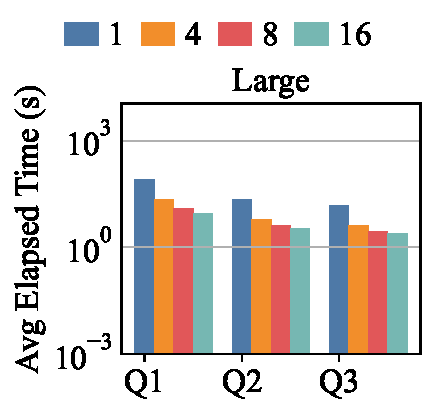
\includegraphics[scale=.6]{parts/architectures/images/query_threads_mimic.pdf}
    \caption{\textsf{MIV}}
\end{subfigure}
\begin{subfigure}[t]{.49\columnwidth}
    \centering
    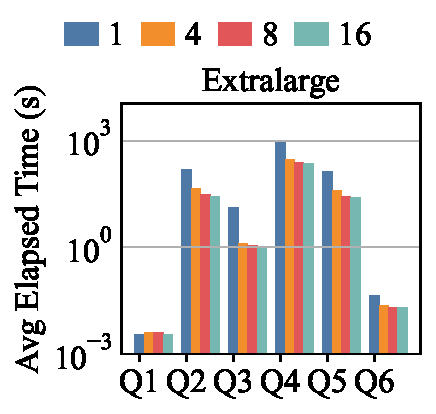
\includegraphics[scale=.6]{parts/architectures/images/query_threads_smartbench.pdf}
    \caption{\textsf{SB}}
\end{subfigure}
\caption{\#Threads speedup ($\uparrow$).}
\label{fig:opt_threads}
\end{figure}

\begin{table}[t]
\centering
\footnotesize
\caption{Average speedups.}
\label{tbl:speedups}
\begin{subtable}[t]{0.52\columnwidth}
\centering
\caption{\#Threads speedup ($\uparrow$).}
\label{tbl:opt_threads}
\setlength{\tabcolsep}{2.5pt}
\renewcommand{\arraystretch}{0.9}
\begin{tabular}{lcccc}
\toprule
 &  & 4 & 8 & 16 \\
Dataset & Size &  &  &  \\
\midrule
\multirow[*]{3}{*}{\textsf{MIV}} & S & 3.3 & 4.2 & 4.5 \\
 & M & 3.7 & 5.5 & 6.3 \\
 & L & 4.0 & 5.8 & 7.3 \\
\midrule
\multirow[*]{4}{*}{\textsf{SB}} & S & 2.8 & 3.7 & 4.3 \\
 & M & 3.2 & 4.0 & 4.6 \\
 & L & 3.6 & 4.3 & 4.9 \\
 & XL & 3.9 & 4.8 & 5.2 \\
\bottomrule
\end{tabular}
\end{subtable}
\hfill
\begin{subtable}[t]{0.42\columnwidth}
\centering
\caption{\#Machines speedup ($\uparrow$).}
\label{tbl:opt_numMachines}
\setlength{\tabcolsep}{2.5pt}
\renewcommand{\arraystretch}{0.9}
\begin{tabular}{lccc}
\toprule
 &  & 2 & 4 \\
Dataset & Size &  &  \\
\midrule
\multirow[*]{3}{*}{\textsf{MIV}} & S & 0.8 & 0.9 \\
 & M & 1.1 & 1.2 \\
 & L & 1.3 & 1.3 \\
\midrule
\multirow[*]{4}{*}{\textsf{SB}} & S & 0.8 & 0.9 \\
 & M & 1.0 & 1.1 \\
 & L & 1.3 & 1.6 \\
 & XL & 1.4 & 2.2 \\
\bottomrule
\end{tabular}
\end{subtable}
\end{table}

\Cref{fig:opt_threads} and \Cref{tbl:opt_threads} summarize the average speedup by increasing the number of execution threads in GS from 1 to 4, 8, and 16.
Speedups are computed using the execution times of \textsc{QueryTSOpt} single-thread implementation (\Cref{tbl:opt_vs_naive}) as the baseline.
For each query, the speedup is calculated as $s_{dataset, size}(x)=\frac{avg_{QID}(\textup{Time with 1 thread})}{avg_{QID}(\textup{Time with x threads})}$, and the values reported in the table correspond to the average speedup across all queries for a given dataset and size.
%Bottom- and top-most speedups are dropped to manage outliers.
Results show substantial benefits from parallel execution, with speedups ranging from approximately 2.8x to 7.3x.
The largest gains are observed on the \textsf{MIV} dataset, where more time-series expose greater opportunities for parallelism.
Overall, the results demonstrate that the proposed implementation scales effectively with the number of threads and that parallelization complements the operator-level optimizations discussed previously.

\subsection{Scaling-out TS: \#Machines}

\begin{figure}[t]
\begin{subfigure}[t]{.49\columnwidth}
    \centering
    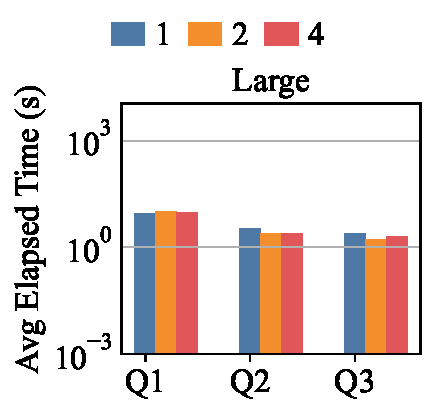
\includegraphics[scale=.7]{parts/architectures/images/query_numMachines_mimic.pdf}
    \caption{\textsf{MIV}}
\end{subfigure}
\begin{subfigure}[t]{.49\columnwidth}
    \centering
    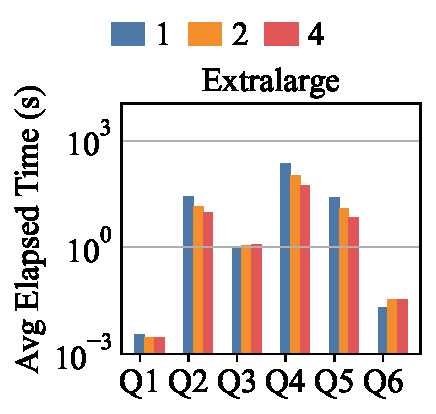
\includegraphics[scale=.7]{parts/architectures/images/query_numMachines_smartbench.pdf}
    \caption{\textsf{SB}}
\end{subfigure}
\caption{\#Machines speedup ($\uparrow$).}
\label{fig:opt_numMachines}
\end{figure}

\Cref{fig:opt_numMachines} and \Cref{tbl:opt_numMachines} summarize the average speedup by increasing the number of machines from 1 to 2 and 4.
Speedups are computed using the execution times of \textsc{QueryTSOpt} single-machine implementation (\Cref{tbl:opt_vs_naive}) as the baseline.
For each query, the speedup is calculated as $s_{dataset, size}(x)=\frac{avg_{QID}(\textup{Time with 1 machine})}{avg_{QID}(\textup{Time with x machines})}$, and the values reported in the table correspond to the average speedup across all queries for a given dataset and size.
%Bottom- and top-most speedups are dropped to manage outliers.
As expected, for small datasets using multiple machines does not provide significant benefits and may even introduce overhead, resulting in speedups less than 1.
However, as dataset size increases, the benefits of distributed execution become more evident, with speedups exceeding 1 and reaching up to 2.2x for the largest \textsf{SB} dataset.
For datasets with shorter time-series (\textsf{MIV}), the speedup from distributed execution is more modest, due to the lower computational demands and the overhead of coordination between machines.

\subsection{Comparison}
\begin{table}[t]
\centering
\footnotesize
\caption{Characteristics of SOTA approaches.}
\label{tab:related_comparisons}
\begin{tabular}{lcccccc}
\toprule
& \multicolumn{2}{c}{Expressiveness} & \multicolumn{2}{c}{Engine} & \multicolumn{2}{c}{Deployment} \\
           \cmidrule(lr){2-3}\cmidrule(lr){4-5}\cmidrule(lr){6-7}
                & Spatial     & Temporal      & Graph     & Time-series   & Distributed   & Persistent \\
\midrule
AGTS            & \ding{51} &           & \ding{51} & \ding{51}     &               & \ding{51}\\
AeonG           &           & \ding{51} & \ding{51} &               &               & \ding{51}\\
HyGraph         &           &           & \ding{51} & \ding{51}     &               &          \\
Neo4J           &           &           & \ding{51} &               &               & \ding{51}\\
\ourapproach    & \ding{51} & \ding{51} & \ding{51} & \ding{51}     & \ding{51}     & \ding{51}\\
\bottomrule
\end{tabular}
\end{table}

\ourapproach is compared against state-of-the-art approaches on temporal graphs and time-series.
\Cref{tab:related_comparisons} summarizes the functional differences among the evaluated systems in terms of spatial and temporal expressiveness, graph and time-series (native) engines, and deployment properties.
Neo4J is a single-model solution based on property graphs.
AeonG~\cite{DBLP:journals/pvldb/HouZWLJWD24} is a native solution for temporal graphs; as in Neo4J, time-series events are treated as graph nodes.
HyGraph~\cite{DBLP:conf/edbt/Ammar0BR25} is a multimodel solution that stores graph and time-series data in-memory (only).
AGTS is a multistore solution extending PostgreSQL with Apache AGE, PostGIS, and TimescaleDB; by relying on PostGIS, it is the only competitor that supports spatial queries.


The comparison is carried out with respect to (1) ingestion, (2) querying, and (3) storage footprint.
Time speedup is computed as $s_{dataset, size}(competitor)=\frac{avg_{QID}(\textup{Competitor Time})}{avg_{QID}(\textup{\ourapproach Time})}$.
$\textup{\ourapproach Time}$ refers to the values of \textsc{QueryTSOpt} in \Cref{tbl:opt_vs_naive} and the values reported in the table correspond to the average speedup across all queries for a given dataset and size.
%Bottom- and top-most speedups are dropped to manage outliers.
Speedup values $>1$ indicate that \ourapproach is faster.
To ensure a fair comparison, all solutions were evaluated under a single-threaded execution environment and average performance is obtained by aggregating twenty experimental runs.
Storage compression is computed as $c_{dataset, size}(competitor)=\frac{\textup{Competitor Storage (MB)}}{\textup{\ourapproach Storage (MB)}}$.
Compression values $>1$ indicate that \ourapproach is more compact.

\textsf{SB}-XL is omitted from the comparison since no competitor was able to load it within the allocated time. 

\subsubsection{Ingestion}

\begin{table}[t]
\centering\footnotesize
\caption{Ingestion and querying speedups with respect to competitors.
\ourapproach is faster if speedup values $>1$.}\label{tab:comparison}
\begin{subtable}[t]{\columnwidth}
\centering
\caption{Ingestion speedup ($\uparrow$).}\label{tab:comp_ing}
\begin{tabular}{lccccc}
\toprule
 &  & AGTS & AeonG & HyGraph & Neo4J \\
Dataset & Size &  &  &  &  \\
\midrule
\multirow[*]{3}{*}{\textsf{MIV}}
& S & \oot$^\dagger$ & 161.4 & 712.5 & \oot$^\dagger$ \\
& M & \oot$^\dagger$ & 184.1 & 812.8 & \oot$^\dagger$ \\
& L & \oot$^\dagger$ & \oot$^\ddagger$ & \oot$^\ddagger$ &   \oot$^\dagger$ \\
\midrule
\multirow[*]{3}{*}{\textsf{SB}}
& S & 2.4 & 241.7 & 0.4 & 64.8 \\
& M & 2.9 & 381.2 & 0.3 & \oot$^\dagger$ \\
& L & 14.9 & \oot$^\ddagger$ & \oot$^\ddagger$ & \oot$^\dagger$ \\
\bottomrule
\end{tabular}
\end{subtable}
\hfill
\begin{subtable}[t]{\columnwidth}
\centering
\caption{Query speedup ($\uparrow$).}
\label{tab:comp_query}
\begin{tabular}{lccccc}
\toprule
 &  & AGTS & AeonG & HyGraph & Neo4J \\
Dataset & Size &  &  &  &  \\
\midrule
\multirow[*]{3}{*}{\textsf{MIV}}
 & S & 2.2 & 5.7 & 9445.5 & 1.6 \\
 & M & 22.3 & 35.3 & 14205.1 & 1.7 \\
 & L & 260.0 & $\ddagger$ & $\ddagger$ & 1.7 \\
\midrule
\multirow[*]{3}{*}{\textsf{SB}}
 & S & 4.3 & 37.7 & 40.7 & 1.8 \\
 & M & 4.5 & 39.9 & 41.7 & 2.1 \\
 & L & 4.8 & $\ddagger$ & $\ddagger$ & 4.8 \\
\bottomrule
\end{tabular}
\end{subtable}
\vspace{1mm}
\footnotesize
\oot: ingestion failed or terminated because more than 500$\times$ slower than \ourapproach.\\
$\dagger$ Bulk loading was used to enable subsequent query experiments. \\
$\ddagger$ No bulk loading is available; no query results could be obtained if ingestion failed.
\end{table}

For both \textsf{MIV} and \textsf{SB}, the ingestion process involves processing a stream of events.
Each event insertion potentially includes getting the corresponding graph node and creating new nodes and edges for time-series events.

\Cref{tab:comp_ing} reports the ingestion performance.
AGTS stores graph structures on top of relational tables.
Consequently, graph insertions incur both graph-layer processing and relational storage overhead.
%, including index maintenance, tuple management, WAL logging, and transactional synchronization.
% This design is less suitable for high-throughput streaming workloads involving large volumes of temporal events.
As a result, high-frequency time-series ingestion workloads become bottlenecked by graph maintenance operations. % rather than raw data insertion throughput. 
Several ingestion attempts for AGTS and Neo4J failed to complete within a reasonable time frame, necessitating the use of bulk loading strategies that are not representative of streaming ingestion performance ($\dagger$ in \Cref{tab:comp_ing}).
AeonG triggers an update for each event insertion, which introduces additional overhead and significantly longer ingestion times; this prevented the possibility to complete the ingestion process for the larger datasets within practical limits ($\ddagger$ in \Cref{tab:comp_ing}).
Finally, while HyGraph's in-memory design allows for high throughput, it fails to scale to larger datasets due to memory constraints, resulting in out-of-memory errors for the larger datasets ($\ddagger$ in \Cref{tab:comp_ing}).

Overall, \ourapproach separates graph from time-series management, allowing events to be efficiently appended independently of graph updates.
This design substantially reduces ingestion costs for persistent baselines and improves scalability; the only speedups below 1 occur against in-memory HyGraph on small and medium \textsf{SB}, which does not provide persistence and fails at larger scales.

\subsubsection{Querying} 

\Cref{tab:comp_query} reports the query performance relative to competing systems.
On the larger datasets, AGTS and Neo4J remain the only comparable baselines among the evaluated competitors, since AeonG and HyGraph could not be queried when ingestion did not complete.
AeonG and HyGraph achieve similar performance in \textsf{SB}, but managing \textsf{MIV} substantially decreases HyGraph performance.
Among the completed runs, \ourapproach maintains a clear advantage over all competitors, with speedups generally increasing as dataset size grows.

\ourapproach becomes increasingly advantageous as dataset size and time-series cardinality grow and is the only system that consistently remains competitive across graph-time-series workloads, demonstrating the effectiveness of its hybrid architecture in combining graph navigation capabilities with efficient temporal data processing.

\subsubsection{Data compression and storage footprint}

\begin{table}[t]
\centering
\footnotesize
\caption{Storage footprint and compression.}
\label{tab:compression}

\begin{subtable}[t]{\columnwidth}
\centering
\caption{
Physical storage footprint of \ourapproach.
GS statistics include only materialized nodes and edges, while TS statistics include time-series events.
Virtual edges (i.e., edges connecting graph nodes and events) are exposed at query time but are not materialized.
Events dominate the logical data volume and storage footprint.
}\label{tab:compression-stgraph}

\resizebox{\columnwidth}{!}{%
\begin{tabular}{lccccccc}
\toprule
& & \multicolumn{3}{c}{GS} & \multicolumn{2}{c}{TS} & \\
\cmidrule(lr){3-5}
\cmidrule(lr){6-7}
Dataset & Size & \#Nodes & \#Edges & Size (MB) & \#Events & Size (MB) & Total (MB) \\
\midrule
\multirow{3}{*}{\textsf{MIV}}& S & $1.3\cdot10^3$ & $6.2\cdot10^2$ & 7.4 &
$1.7\cdot10^6$ & 70 & 77 \\
& M & $1.3\cdot10^4$ & $6.6\cdot10^3$ & 74 &
$1.7\cdot10^7$ & 698 & 772 \\
& L & $1.3\cdot10^5$ & $6.5\cdot10^4$ & 734 &
$1.7\cdot10^8$ & 6949 & 7683 \\
\midrule
\multirow{4}{*}{\textsf{SB}}& S & $3.4\cdot10^{3}$ & $6.7\cdot10^{3}$ & 2.1 &
$2.5\cdot10^{6}$ & 60 & 62 \\
& M & $6.0\cdot10^{3}$ & $1.2\cdot10^{4}$ & 4.6 &
$1.0\cdot10^{7}$ & 234 & 239 \\
& L & $2.6\cdot10^{4}$ & $5.5\cdot10^{4}$ & 16 &
$2.6\cdot10^{8}$ & 5795 & 5811 \\
& XL & $6.0\cdot10^{3}$ & $1.2\cdot10^{4}$ & 4.6 &
$3.0\cdot10^{8}$ & 6332 & 6336 \\
\bottomrule
\end{tabular}}
\end{subtable}

\begin{subtable}[t]{\columnwidth}
\centering
\caption{Compression with respect to competitors.
\ourapproach is more compact if compression values $>1$.}
\label{tab:compression-competitors}
\begin{tabular}{lccccc}
\toprule
Dataset & Size & AGTS & AeonG & HyGraph & Neo4J \\
\midrule
\multirow{3}{*}{\textsf{MIV}}
 & S & 2.4 & 7.6 & $\dagger$ & 4.2 \\
 & M & 2.4 & 7.6 & $\dagger$ & 4.4 \\
 & L & 2.4 & $\ddagger$ & $\ddagger$ & 4.3 \\
\midrule
\multirow{3}{*}{\textsf{SB}}
 & S & 10.8 & 9.4 & $\dagger$ & 7.8 \\
 & M & 10.9 & 8.4 & $\dagger$ & 7.5 \\
 & L & 11.5 & $\ddagger$ & $\ddagger$ & 7.5 \\
\bottomrule
\end{tabular}
\\
$\dagger$ In-memory. \\
$\ddagger$ No bulk loading is available; no data was stored (see \Cref{tab:comparison}).
\end{subtable}
\end{table}

\ourapproach does not materialize edges toward individual events; instead, events are accessed through virtual edges that are generated at query time.
As the number and length of time-series increase, this significantly reduces storage footprint.
\Cref{tab:compression-stgraph} shows the effectiveness of the hybrid storage layout and the physical separation between graph and time-series data.
Storage grows approximately linearly with the number of temporal events: for instance, in the MIV dataset, increasing the event count from $1.7\cdot10^6$ to $1.7\cdot10^8$ results in a growth from 77 MB to 7.7 GB. 
The time-series storage (TS) dominates the overall footprint, accounting for more than 90\% of the total space in all datasets, while the graph structure (GS) remains comparatively small.
When compared to the original datasets (\Cref{tab:datasets}), \ourapproach saves up to $10^4$ times in terms of stored edges.

\Cref{tab:compression-competitors} reports the compression ratio with respect to competitors and it shows that \ourapproach remains substantially more compact than alternative systems, achieving compression factors between $2.4\times$ and $11.5\times$.
The largest gains are observed on the SB datasets, where \ourapproach requires up to an order of magnitude less space than AGTS, AeonG, and Neo4J.
Furthermore, several large instances cannot be managed by AeonG or HyGraph.

\section{Conclusion and future directions}\label{sec:conclusion}

This paper introduced \ourapproach, a multistore system for managing spatio-temporal property graphs whose data combine slowly evolving graph structures with high-volume time-series.
\ourapproach exposes a unifying spatio-temporal property graph abstraction while physically separating graph nodes and edges, stored in GS, from time-series events, stored in TS.
The connection between the two stores is provided at query time through virtual edges, avoiding the materialization of one graph edge per event.
\ourapproach supports temporal validity for nodes, edges, and properties, and rewrites query plans so that event-local operators can be pushed down to TS.
The experimental evaluation shows that this design reduces storage overhead, improves ingestion, and accelerates analytical queries with respect to single- and multimodel and multistore baselines.

Several research directions remain open.
\ourapproach 
(i) currently supports conjunctive path queries, adding regular path queries would enable more expressive graph navigation while introducing new opportunities for cross-store optimization;
(ii) follows the property-graph paradigm, enriching it with native time-series operators would allow users to combine graph traversal and temporal analytics within a unified model;
(iii) currently optimizes single-access time-series queries, a global optimizer capable of jointly reasoning about multiple time-series operations could further improve execution efficiency;
(iv) targets historical queries, supporting streaming graph-time-series workloads would enable real-time monitoring and decision-making over continuously evolving data.


\begin{partsummary}

This part addressed the first two steps of the progression outlined at the close of \Cref{chap:data_oriented_perspective}: proposing a general-purpose schema for the data architecture of a Digital Twin, and proposing a data model, and a consequent system to manage, integrate and represent Digital Twin data.

\Cref{chap:dataplat} addressed the first step, through the design of a data platform for the AGRITECH precision agriculture case study. The requirements identified there, arising directly from the volume, variety, velocity, and veracity of the data produced by six independently developed research activities, motivated a reference architecture organized around independent, composable modules -- ingestion, storage, data processes, management, and exploitation -- together with a domain-level conceptual schema generalizing the entities recurring across these activities into agents, environments, measurements, and tasks. \Cref{chap:datamodel-dt} addressed the second step, showing that implementing this conceptual schema relationally exposes two difficulties characteristic of Digital Twin data more generally: the dynamic, time-varying relationships among entities, which relational schemas can only represent through proliferating association tables, and the rigidity such schemas impose on later extension. STGraph, the multistore system presented in that chapter, addressed both difficulties by representing entities and their evolving relationships as a spatio-temporal property graph, while delegating the high-volume time-series data such entities produce to a dedicated time-series store connected to the graph through virtual edges.

Once a Digital Twin's data is integrated and represented through this reconciled layer, it becomes possible to explore the functionality such integration newly enables; \Cref{part:methods-applications} does so directly, illustrating applications built on top of the platform and data model presented in this part. At the same time, the growing complexity of these data representations, and of the infrastructure required to support them, raises a complementary question: how such complexity can be managed, and made tractable for the humans who must still interact with it. \Cref{part:methods-applications} also explores methods addressing this question, aimed at easing human interaction with increasingly complex data representations and the systems built around them.

\end{partsummary}